\graphicspath{{Figures/}}
\newcommand{\proportional}{\mathbf{P}}
\newcommand{\derivative}{\mathbf{D}}
\chapter{Preliminaries and State-of-the-Art} \label{chap:background}
%In this chapter, we will present the Quadratic Programming (QP) formulation used 
  
In this chapter, we present prior knowledge of task-space control and how it can be formulated using Quadratic Programming (QP). That is to say, a brief review of the meaning of tasks as part of the cost function and the constraints with different schemes of multi-objective QP control. After that, we discuss the different approaches dealing with the stability and robustness of QP control schemes. An overview of robotic applications that successfully make use of QP control is also given.
%The motivation of this paper came first some experimental failures. In the context of aircraft manufacturing robotics~\cite{kheddar2019ram}, we shall demonstrate the capability of humanoid robots in accessing narrow, cumbersome or confined spaces. In one specific use-case, our QP controller~\cite{bouyarmane2019tro} repeatedly failed in the course of the execution at an extreme configuration. The log data revealed that similar failures happened when the joints reached their bounds, or in cases where joint velocities were too high. We also discovered later on that the QP either failed or generated oscillatory and discontinuous motions in closed-loop for other bounds (e.g. collision avoidance). Similar experimental failures encountered in closed-loop control have been reported in~\cite{johnson2015journalOfFieldRobotics}. 
\section{Quadratic Programming}
Optimization problems aim at finding the best parameters $\decisionVector$ that minimize a criterion called cost-function while not violating a set of constraints. Quadratic Programming (QP) is a particular case of optimization problems where the cost-function is quadratic and the (equality and inequality) constraints are linear w.r.t $\decisionVector$, respectively~\cite{betts2010bookOptimalControl}. The general form of QP is 
\begin{align}\label{eq-chap0:QP general form}
	\begin{split}
		\underset{\decisionVector}{\min}& \fracOneTwo \decisionVector\tp\mathbf{H}\decisionVector + \bm{h}\tp\decisionVector\\
		\text{s.t: }& \mathbf{C}_{\rm eq} \decisionVector = \bm{d}_{\rm eq}\\
					& \mathbf{C}_{\rm ineq} \decisionVector \leq \bm{d}_{\rm ineq}
	\end{split}.
\end{align}
If the Hessian matrix $\mathbf{H}$ is  positive semi-definite then QP is convex~\cite{nocedal2006springerBookOPtimization}. The space within which the QP is solved is called the feasibility domain. Least-square minimization is also an optimization problem that minimizes the 2-norm of a vector that is affine in terms of $\decisionVector$ while satisfying a set of affine constraints set similarly to \cref{eq-chap0:QP general form}. The least-square minimization is expressed as  
\begin{align}\label{eq-chap0:least-square general form}
	\begin{split}
		\underset{\decisionVector}{\min}& \fracOneTwo \norm{\mathbf{A}\decisionVector+\bm{b}}_\mathbf{W}^2\\
		\text{s.t: }& \mathbf{C}_{\rm eq} \decisionVector = \bm{d}_{\rm eq}\\
		& \mathbf{C}_{\rm ineq} \decisionVector \leq \bm{d}_{\rm ineq}
	\end{split},
\end{align}
where $\mathbf{W}$ is a positive-semi-definite weighting matrix\footnote{If $\mathbf{W} = \eye$ then weighting subscript is dropped.}. Least-square minimization \cref{eq-chap0:least-square general form} can be cast to convex QP such that
$\mathbf{H} = \mathbf{A}\tp\mathbf{W}\mathbf{A}$ (assuming non-singular $\mathbf{A}$ \cite{ayres1962schaum}) and $\bm{h} = \mathbf{A}\tp\mathbf{W}\bm{b}$. However, the vice-versa is in general not true\footnote{This is only possible if $\bm{h}\in{\rm Im}\left\{\mathbf{H}\right\}$.}. In robotics control context, QP often  originates from a least-square problem since the resulting cost-function has a more \emph{practical} sense (i.e., find $\decisionVector$ that makes $\mathbf{A}\decisionVector$ as close as possible to $-\bm{b}$ while satisfying all the constraints) than just an abstract quadratic form.   

The existing algorithms to solve convex QP with equality and inequality constraints are based mainly on two approaches: \emph{active-set} and \emph{interior-point} methods. They differ in the way inequality constraints are handled. In addition, the former is suited for small and medium-size problems, whereas the latter is more efficient for large-size problems. Nevertheless, the active-set method convergence can be greatly improved if an estimate of the solution is available, commonly called the ‘warm-start.’ In control applications, QP has to be solved online at each control step. The QP solution of the previous iteration can then be used as a warm-start for the current one, which makes active-set methods preferable in such a context. Exploiting the warm-start option for interior-point methods is still ongoing research. For more discussion about QP solving algorithms, please refer to \cite[Chapter 16]{nocedal2006springerBookOPtimization}.  
  
\section{Robot Kinematics and Dynamics}
A robot is a set of links (bodies) connected through joints that are free to move along their Degree-of-Freedom (DoF). A joint is active (actuated) if it is equipped with an actuator that generates a torque that changes its position and velocity. Otherwise, it is called passive. We refer to \emph{task-space} as the space in which the state of a certain point of interest $\fkin(\genActConf)\inR^m$ is monitored (e.g., position and orientation of a body, robot Center-of-Mass (CoM) in Cartesian space, position of an object in the robot Field-of-View (FoV)), whereas \emph{configuration-space} denotes the space in which the robot configuration $\genActConf$ is defined. %Generally, the mapping between the task-space and joint-space is non-linear. 
We consider the general case of a floating-base robot such that 
\begin{equation}\label{eq-chap0:gen act conf formal form}
	\genActConf = \left(\FB,\actConf\right)\in SE(3)\times\mathbb{R}^n,
\end{equation}
where $\FB\in SE(3)$ is the position and orientation of the floating-base, $\actConf\in\mathbb{R}^n$ is the joint positions vector defined in the \emph{joint-space} and $n\in\mathbb{N}$ denotes the actuated DoF.  For convenience, we rewrite $\genActConf$ in~\cref{eq-chap0:gen act conf formal form} as a vector form
\begin{equation}\label{eq-chap0:gen act conf def}
	\genActConf\tp = \begin{bmatrix}
		\FB\tp & \actConf\tp
	\end{bmatrix}\in\mathbb{R}^{{7+n}}, \ 
	\genActConfDot\tp = \begin{bmatrix}
		\FBDot\tp & \actConfDot\tp %\dot{\actConf}^T
	\end{bmatrix}\in\mathbb{R}^{6+n},
\end{equation}
where $\FB=\begin{bmatrix}
	\bm{p}^{\rm FB}  \\ \quaternion^{\rm FB}
\end{bmatrix}\inR^{7}$ is the floating-base pose (position $\bm{p}^{\rm FB} \inR^3$ and  orientation $\quaternion^{\rm FB}\inR^4$ parameterized with unit quaternion) and $\genActConfDot$ is the robot state  velocity such that $\FBDot\inR^6$ is the floating-base velocity and and $\actConfDot\inR^n$ is the joint velocity. 
\begin{remark}\label{rem:fixed-base robot}
	A fixed-base robot is considered as a special case such that $\genActConf = \actConf$, $\genActConfDot = \bm{\dot{\genActConf}} = \actConfDot$ and $\genActConfDDot = \bm{\ddot{\genActConf}} = \actConfDDot$. The configuration-space and joint-space are equivalent. 
\end{remark}
\noindent
$\genActConfDot$ is linearly mapped to $\fkinDot\inR^m$ through the Jacobian $\jac\inR^{m\times(6+n)}$ such that (the dependency on $\genActConf$ is dropped for ease of reading)
\begin{equation}
	\fkinDot = \jac\genActConfDot,
\end{equation}
and whose time derivative is 
\begin{equation}
	\fkinDDot = \jac\genActConfDDot + \jacDot\genActConfDot.
\end{equation}
The Equation of Motion (EoM) that governs the robot dynamics in the presence of contact is 
\begin{equation}\label{eq-chap0:equation of motion}
	\massMat(\genActConf)\genActConfDDot + \nnLinTorqueMat(\genActConf,\genActConfDot)\genActConfDot + \gravity(\genActConf) = \selectMat\Tau + {\actJacContact}\tp\force,
\end{equation} 
with $\massMat\inR^{(6+n)\times(6+n)}$ is the mass matrix, $\nnLinTorqueMat^{(6+n)\times(6+n)}$ is the Coriolis-centrifugal matrix, $\gravity\inR^{(6+n)}$ denotes the gravitational torque, $\selectMat\tp=\begin{bmatrix}
	\zeros & \eye
\end{bmatrix}\inR^{n\times (6+n)}$ is the actuated DoF selection matrix, $\actJacContact\inR^{3\times (6+n)}$ is the Jacobian at the contact point and $\force\inR^3$ is the frictional contact force\footnote{For clarity, the dependencies on $\genActConf$ and $\genActConfDot$ are omitted.}.

In the next section, we discuss task-space control and how it can be formulated as a QP.
\section{Task-Space Control}
Task-space control consists of finding  $\genActConfDDot$ (equivalently $\Tau$ from \cref{eq-chap0:equation of motion}) that brings $\fkin$ to a reference target $\fkinRef$.
Let us assume that there exists a task-space feedback $\taskCrtlIn$\footnote{The way how $\taskCrtlIn$ can be formulated is discussed in  \cref{subsec-chap0:task formulation}.} such that if 
\begin{align}\label{eq-chap0:task-space control}
	\fkinDDot = \jac\genActConfDDot + \jacDot\genActConfDot= \taskCrtlIn
\end{align} than the task error $\bm{e} = \fkin - \fkinRef$ converges to zero\footnote{This is described as  the task-function approach coined in \cite{samson1990ifac,samson1991book}}.
From \cref{eq-chap0:task-space control}, the inverse problem can be solved using  QP 
\begin{align}\label{eq-chap0:simplest QP}
	\begin{split}
	&\underset{\genActConfDDot}{\min}\fracOneTwo \norm{\genActConfDDot}^2 \\ 
	\text{s.t: }&  \jac\genActConfDDot + \jacDot\genActConfDot= \taskCrtlIn
	\end{split}.
\end{align} 
The solution of QP \cref{eq-chap0:simplest QP} is equivalent to the Jacobian-null-space-projection formulation~\cite{dietrich2015ijrr} 
\begin{equation}\label{eq-chap0:null-space projection}
	\genActConfDDot = \jac^{+}\left(\taskCrtlIn- \jacDot\genActConfDot\right),
\end{equation} where $\jac^+ = \jac\tp\left(\jac\jac\tp\right)\inv$ is the Jacobian pseudo-inverse.
However, if the Jacobian $\jac$ is non-square with $(6+n)>m$, then there exists an infinity of $\genActConfDDot$ that corresponds to the same $\fkin$. This is related to the notion of redundancy: a robot is redundant if it has more DoF than what is strictly required to perform a given task~\cite{deluca1991springer,chiaverini1991roboticsandAutonomousSystems,antonelli1998icra,chiaverini2019springer}. For example, to control a body pose, the task dimension $m=6$. Not surprising that most modern robotic manipulators and humanoid arms have at least 7 DoF (similar to the human anatomy~\cite{chiaverini1991ras}). 
The non-uniqueness of $\genActConfDDot$ means that some DoF are not needed to perform the task \cite{wieber2017springer}, and this induces two undesirable behaviors: (i) non-repeatability of the robot configuration for the same task-space mapping; and (ii) null-space motion\footnote{The null-space motion denotes the remaining redundancies that live in the null-space of the task Jacobian and thereby do not perturb $\fkin$. They are also known as the zero-dynamics~\cite{varghese1990icse,varghese1991taes}.}~\cite{deluca1991springer}. To mitigate these issues, a secondary task can be performed to solve the remaining redundancies. In particular, QP \cref{eq-chap0:simplest QP} can rewritten as 
\begin{align}\label{eq-chap0:2tasks QP}
	\begin{split}
		&\underset{\genActConfDDot}{\min}\fracOneTwo \norm{\genActConfDDot-\boldsymbol{\mu}^*}^2 \\ 
		\text{s.t: }&  \jac\genActConfDDot + \jacDot\genActConfDot= \taskCrtlIn
	\end{split}.
\end{align}
where $ \boldsymbol{\mu}^*$ is a feedback that brings the robot joints as close as possible to a desired configuration (e.g., elbow-up configuration). Similarly to  \cref{eq-chap0:simplest QP,eq-chap0:null-space projection}, the closed-form solution of QP \cref{eq-chap0:2tasks QP} is~\cite{siciliano1991icar} 
\begin{equation}\label{eq-chap0:null-space projection 2tasks}
%	\genActConfDDot = \jac^+\left(\taskCrtlIn- \jacDot\genActConfDot\right) + \left(\eye - \jac^+\jac\right)^{+}\genActConfDDot^*,
	\genActConfDDot = \left(\eye + \mathbf{P}^{+} \right)\jac^+\left(\taskCrtlIn- \jacDot\genActConfDot\right) - \mathbf{P}^{+} \boldsymbol{\mu}^*,
\end{equation} 
with $\mathbf{P}= \left(\eye - \jac^+\jac\right)$ is the Jacobian-null-space projector.

In general, other control objectives\footnote{A control objective is a generic term to encompass both tasks and constraints.} expressed as unilateral and bilateral constraints have  to be accounted for as (\cref{fig:HRP4-task-constraints}):
\begin{itemize}
	\item Torque bounds: 
	\begin{equation}\label{eq-chap0:tau bounds}
		\selectMat\Tau_{\min}\leq  	\massMat\genActConfDDot + \nnLinTorqueMat\genActConfDot + \gravity - {\actJacContact}\tp\force \leq\selectMat\Tau_{\max}.
	\end{equation} 
	\item Acceleration bounds: 
	\begin{equation}\label{eq-chap0:acceleration bounds}
		\boldsymbol{\dot{\alpha}}_{{\bm{q}}_{\min}}\leq
		\genActConfDDot
		\leq\boldsymbol{\dot{\alpha}}_{{\bm{q}}_{\max}}.
	\end{equation}
	\item Contact forces inside the friction cone: 
	\begin{equation}\label{eq-chap0:force constraint}
		\force \in{\cal K}, 
	\end{equation} which can be expressed in the linearized form
	\begin{equation}\label{eq-chap0:force constraint linearized}
		\force = \mathbf{R}\boldsymbol{\beta}, \ \boldsymbol{\beta}\tp=\begin{bmatrix}\beta_1\ldots\beta_{\gls{nFricCone}}\end{bmatrix}, \ \beta_{i}\geq0,
	\end{equation}
	with $\mathbf{R}=\begin{bmatrix}
		\boldsymbol{\rho}_1 & \ldots & \boldsymbol{\rho}_{\gls{nFricCone}}
	\end{bmatrix}\inR^{3\times\gls{nFricCone}}$ where $\boldsymbol{\rho}_j\in\mathbb{R}^3$ is the $j^{\text{th}}$ vertex of the linearized friction cone.% and  $\boldsymbol{\beta}\inR^{\gls{nFricCone}}$ is the vector of positive coefficients.
	\item Non-slipping contact: 
	\begin{equation}\label{eq-chap0:non-slipping contact}
		\actJacContact\genActConfDDot + \actJacContactDot \genActConfDot = \zeros
	\end{equation}
	\item A set of constraints in the form: 
	\begin{equation}\label{eq-chap0:gen form kinematic constraint}
		H(\genActConf,\genActConfDot)\geq 0 
	\end{equation}
	where $H(\genActConf,\genActConfDot)$ can express different distance and velocity constraints, such as: 
	\begin{itemize}
		\item Joint position bounds:
		\begin{equation}\label{eq-chap0:joint position constraint}
			\genActConf_{\min}\leq\genActConf\leq \genActConf_{\max}.
		\end{equation}
		\item Joint velocity bounds:
		\begin{equation}\label{eq-chap0:joint velocity constraint}
			\boldsymbol{\alpha}_{{\mathbf{q}}_{\min}}\leq\genActConfDot\leq \boldsymbol{\alpha}_{{\mathbf{q}}_{\max}}.
		\end{equation}
		\item CoM  inside the equilibrium region or any other constraint eventually implying CoM velocity~\cite{audren2018tro}:
		\begin{align}\label{eq-chap0:com constraints}
			\bm{ CoM}(\genActConf)&\in {\cal P} \;\; {\rm or} \;\; \bigcup \; \bm{ CoM}(\genActConf)\leq \Delta,\\ 
			\bm{\dot{CoM}}_{\min}&\leq\bm{\dot{CoM}}(\genActConf,\genActConfDot)\leq \bm{\dot{CoM}}_{\max}.
		\end{align}
		\item Collision avoidance constraint~\cite{vaillant2016springer,vaillant2016trvcg}:
		\begin{equation}\label{eq-chap0:generic distance constraint}
			\delta(\genActConf)\geq\delta_{\min},
		\end{equation}
		where $\delta(\genActConf)$ is the distance to the collision.
		\item Body velocity $\bm{v}_{\rm body}$ bounds:
		\begin{equation}
			\bm{v}_{\rm body}(\genActConf,\genActConfDot) \leq \bm{v}_{\max}.
		\end{equation}
		\item  FoV  inclusion constraints in visual servoing or vision-based object tracking~\cite{paolillo2018ral}. One needs to keep the object of interest $\cal O$ within the FoV of the robot embedded camera, and out of any known possible occlusions. These are linked to the robot configuration:
		\begin{equation}
			FoV(\genActConf) \ni {\cal O}.
		\end{equation} The inclusion is also  written equivalently into a set of inequalities, see e.g.,~\cite{agravante2017ral}.
	\end{itemize}
and possibly others.
\end{itemize}

Even though  \cref{eq-chap0:null-space projection 2tasks} has been generalized to $N$ tasks in \cite{siciliano1991icar}, unilateral constraints cannot be straightforwardly accounted for in the  Jacobian-null-space-projection approach, and alternative solutions have been proposed. 
%especially for distance constraints (joint position limits, collision avoidance, etc...). 
Using \cref{eq-chap0:null-space projection 2tasks}, \cite{liegeois1977tsmc} formulated a secondary task that minimizes the deviation of the joints from the middle of their available range.~\cite{schwienbacher2011icra} added a term to the secondary task that repels the joint from its boundaries. However, if there are no redundancies left from the primary task, collision with joint limits cannot be avoided. 
 
Artificial Potential Field proposed by \cite{khatib1985icra} allowed to assign the same priority level to perform the reaching motion and collision avoidance. The total force applied to the end-effector derives from the sum of a decreasing artificial field toward the target and an increasing one near the obstacle. This approach was further improved in~\cite{dietrich2011icra} by adding a dissipative term. However, this method may get stuck into local minima and oscillations, especially when the robot attempts to go through two opposite obstacles~\cite{singletary2021iros}. In addition, it is often non-desired to have a repulsive behavior w.r.t the obstacle as this may significantly reduce the robot's workspace. 

Stack-of-tasks framework \cite{mansard2009tro}  has been proposed to consider unilateral constraints as equality constraints if the robot is close enough to the obstacle. Indeed, it allows exploiting \cref{eq-chap0:null-space projection 2tasks} where collision avoidance is the primary task. However, it has been shown that the approach does not scale well when several constraints are approaching their limits. 

\cite{flacco2012icra} proposed an algorithm that sophistically solves redundancy while satisfying joint limits. By solving the Inverse-Kinematics (IK) problem, the algorithm saturates recursively the joint velocities that exceed their bounds and finds the possible remaining redundant-solutions that achieve the task at best. However, the algorithm may perform several null-space projections for yet one solution, which can be time-consuming, especially in high DoF robots like humanoids. In addition, kinematic constraints that are not defined in joint-space are conservatively handled.

 As a last resort, unilateral constraints can be processed after computation which inevitably leads to sub-optimal solutions~\cite{baerlocher2004visualComputer,kim2016humanoids,feng2013humanoids}.
\begin{figure}
	\centering
	\includegraphics[width = 0.65\columnwidth]{HRP4-task-constraints}
	\caption{Multi-objective control: HRP-4 robot right hand reaching a Cartesian target while being subject to several unilateral constraints.}
	\label{fig:HRP4-task-constraints}
\end{figure}
\subsection{QP-based Task-Space Control Formulation}\label{subsec-chap0:task-space QP}
QP naturally handles inequality constraints, which is the main factor for its use in robot control. As shown in \cref{eq-chap0:QP general form,eq-chap0:least-square general form}, satisfying unilateral constraints is systematically given a high priority over the control objectives defined in the cost-function. %This matches intuitively with how the control objectives can be sorted. 
The first premise of QP-based controllers accounting for the collision avoidance constraint dates back to \cite{faverjon1987icra}. The computer processor units available at the time did not enable a real-time application on the robot\footnote{The reported QP computation time was 10 times higher than the required real-time constraint.}. However, the simulation showed how the robot collision with multiple obstacles --a behavior that is difficult to obtain with \cite{khatib1985icra} approach. 

After that, QP has been formulated for redundancy resolution while accounting for joint position, velocity, acceleration and torque bounds~\cite{cheng1994tra,park1998icra,zhang2004transactionsonSysManCyb1,zhang2004transactionsonSysManCyb2,zhang2006icrb}. These approaches formulated IK-QP  where $\decisionVector=\genActConfDot$. In addition, the control scenario was quite simple, where a reaching motion is performed while satisfying the unilateral constraints. 

In order to perform more complex and dynamically consistent tasks, Inverse-Dynamics (ID) QP controllers has been formulated to perform dynamic balance, locomotion, manipulation, grasping, and multi-frictional contact~\cite{abe2007siggraph,collette2007humanoids,macchietto2009siggraph,delasa2010trGraph,salini2011icra,salini2010springer,bouyarmane2011iros,saab2011icra}. In almost all existing ID-QP controllers, the decision variable vector $\decisionVector$ encompasses the robot state acceleration $\genActConfDDot\inR^{6+n}$ and the contact forces $\force\in\mathbb{R}^3$
\begin{equation}\label{eq:decision variables vector}
	\decisionVector = \begin{bmatrix}
		\genActConfDDot \\ \force
	\end{bmatrix}\inR^{n+9}.
\end{equation}
Given that the constraints \cref{eq-chap0:tau bounds,eq-chap0:acceleration bounds,eq-chap0:force constraint} are affine in terms of $\decisionVector$, the ID task-space QP controller is formulated as
%\begin{subequations}\label{eq-chap0:inverse-dynamics QP}
\begin{align}\label{eq-chap0:inverse-dynamics QP}
	\begin{split}
		\underset{\decisionVector}{\min}& \fracOneTwo \norm{\mathbf{A}\decisionVector+\bm{b}}^2\\
		\text{s.t: }& \selectMat\Tau_{\min}-\nnLinTorqueMat\genActConfDot-\gravity\leq\begin{bmatrix}
			\massMat & - {\actJacContact}\tp
		\end{bmatrix}\decisionVector \leq \selectMat\Tau_{\max} -\nnLinTorqueMat\genActConfDot-\gravity\ \\ 
		& \boldsymbol{\dot{\alpha}}_{{\bm{q}}_{\min}}\leq
		\begin{bmatrix}
			\eye & \zeros
		\end{bmatrix}\decisionVector
		\leq\boldsymbol{\dot{\alpha}}_{{\bm{q}}_{\max}} \\ 
		&\begin{bmatrix}
			\zeros&\eye 
		\end{bmatrix}\decisionVector \in \cal K \\ 
	&\begin{bmatrix}
		\actJacContact&\zeros
	\end{bmatrix}\decisionVector =- \actJacContactDot \genActConfDot
		%{ \rm \cref{eq-chap0:tau bounds,eq-chap0:acceleration bounds,eq-chap0:force constraint}}
	\end{split}.
\end{align}
%\end{subequations}
The constraints in QP~\cref{eq-chap0:inverse-dynamics QP} play the role of a filter for the solution $\decisionVector$: if the  cost-function minimum $\decisionVector_{\rm cost-func \min}$ is inside the constraint set then $\decisionVector = \decisionVector_{\rm cost-func \min}$. Otherwise, $\decisionVector_{\rm cost-func \min}$ is filtered such that $\decisionVector$ is chosen to be the closest point to $\decisionVector_{\rm cost-func \min}$ among the constraint set.
 
The velocity and distance constraints class \cref{eq-chap0:gen form kinematic constraint} cannot be directly included in QP \cref{eq-chap0:inverse-dynamics QP} since they are not expressed in terms of $\decisionVector$. This class of constraints needs special consideration. Seeking a formulation that expresses these kinematic constraints in terms of $\decisionVector$ may be vague and devoid of any physical meaning. A more correct question would be \emph{how to choose/formulate an affine constraint on $\decisionVector$ such that the kinematic constraints are satisfied forward in time?} In addition, we may ask the relatively same question about how to formulate task-space feedback $\taskCrtlIn$ to steer the task state $\fkin$ toward $\fkinRef$. 
These two points are discussed in the next section.
%As shown in \cref{eq-chap0:QP general form,eq-chap0:least-square general form}, satisfying unilateral constraints is systematically given a high priority over the cost-function minimization. This matches intuitively with how the the control objectives can be sorted. 
%In general, we are be interested into  driving $\bm{e}$ to zero while being as close as possible  t keeps a point of interest inside a given set. 

%The ability to perform multi-tasks requires subsequently to assign a priority level for each task. For instance, QP formulation  in \cref{eq-chap0:2tasks QP} shows that the secondary posture task is achieved at best while not perturbing the primary task (steering $\bm{e}$ to zero). In the next section \cref{...}, we will discuss other existing prioritization schemes where more than two tasks can be performed. 



\section{Tasks and Kinematic Constraints Formulation}\label{sec-chap0:Task and Kinematic Constraints Formulation}
In this section, we go through the state-of-the-art formulations of the tasks-space feedback and kinematic constraints in terms of $\decisionVector$. The pro and cons of these approaches are also discussed. 
\subsection{Task Formulation}\label{subsec-chap0:task formulation}
 If for a given task-space reference target $\fkinRef$ we have the corresponding  configuration $\refConf$ such that $\fkin(\refConf) = \fkinRef$, than the control problem would be simply to make $\genActConf$ converge toward  $\refConf$. Unfortunately, the mapping between task-space and configuration-space is often nonlinear preventing from easily solving  the inverse-geometric problem. Instead, nonlinear control techniques can be used, especially \emph{feedback linearization}~\cite{slotine1991applied,khalil2002NonLinearSystems}. The idea consists in constructing a linear system in the task-space based on the successive derivatives of $\fkin$\footnote{Conversely to $\fkin$, $\fkinDot$ and $\fkinDDot$ are linear w.r.t $\genActConfDot$ and $\genActConfDDot$. }
 \begin{align}\label{eq-chap0:task dynamics}
 	\begin{split}
 		\actTaskOutDot = \underset{\AactTaskOut}{\underbrace{\begin{bmatrix}
 					\zeros & \eye \\ \zeros & \zeros  
 		\end{bmatrix}}}\actTaskOut + 
 		\underset{\BactTaskOut}{\underbrace{\begin{bmatrix}
 				\zeros \\ \eye
 		\end{bmatrix}}} \taskCrtlIn, \ 
 	\actTaskOut = \begin{bmatrix}
 		\bm{e} \\ \bm{\dot{e}}
 	\end{bmatrix} = 
 	\begin{bmatrix}
 		\fkin - \fkinRef \\ \fkinDot - \fkinRefDot
 	\end{bmatrix}\inR^{2m}, 
 	\end{split}
 \end{align} 
where $\fkinRef,\fkinRefDot,\fkinRefDDot\inR^{m}$ are the reference terms of a trajectory to be tracked, and $\actTaskOut$ is the task state vector.
 Next, a feedback $\taskCrtlIn$ is formulated to steer $\bm{e},\bm{\dot{e}}$ and $\bm{\ddot{e}}$ to zero. %toward $\fkinRef$. 
 Then, $\taskCrtlIn$ is mapped to the configuration-space control input (either $\genActConfDDot$ or $\Tau$)
 \begin{equation}\label{eq-chap0:task feedback mapped to alphaD and tau}
 	\taskCrtlIn = \jac\genActConfDDot + \jacDot\genActConfDot = \jac\massMat\inv\selectMat\Tau +  \left(\jacDot - \jac\massMat\inv\nnLinTorqueMat\right)\genActConfDot - \jac\massMat\inv\gravity.
 \end{equation}
Since \cref{eq-chap0:task feedback mapped to alphaD and tau} is affine w.r.t $\genActConfDDot$, it can be integrated in the cost-function of QP \cref{eq-chap0:inverse-dynamics QP} as $\norm{ \jac\genActConfDDot + \jacDot\genActConfDot- \taskCrtlIn }^2$.
\subsubsection{Proportional-Derivative Controller}
Given the task dynamics in \cref{eq-chap0:task dynamics}, the simplest way to formulate $\taskCrtlIn$ is through a Proportional-Derivative (PD) feedback \cite{abe2007siggraph,westervelt2007book,nakanishi2008ijrr,macchietto2009siggraph,delasa2010trGraph,galloway2015ieeeAccess,bouyarmane2018tac,kolathaya2019iros,englsberger2020rss}
\begin{equation}\label{eq-chap0:task feedback}
	\taskCrtlIn = \fkinRefDDot - \taskStiffness\actOut - \taskDamping	\actOutDot,
\end{equation}
with $\taskStiffness,\taskDamping\inR^{m\times m}$ are the stiffness and damping gain matrices. By replacing \cref{eq-chap0:task feedback} into \cref{eq-chap0:task dynamics}, we get the closed-loop task dynamics
\begin{equation}\label{eq-chap0:closed-loop task dynamics}
	\actOutDDot + \taskDamping\actOutDot + \taskStiffness\actOut = 0.
\end{equation}  
Given \cref{eq-chap0:closed-loop task dynamics}, $\taskStiffness$  and $\taskDamping$ are simply required to be positive-definite to ensure asymptotic $\actTaskOut$ convergence to the origin~\cite{khalil2002NonLinearSystems}. Generally, they are taken as diagonal matrices to ensure a decoupled convergence of the task error coordinates.  

\cref{eq-chap0:closed-loop task dynamics} shows that the task error dynamics is similar to a mass-spring-damper. Impedance control is based on the same policy, except that the mass is not equal to unity but equal to the task-space projected mass matrix~\cite{dietrich2016ral,dietrich2017ral,dietrich2020tro,englsberger2020rss}. PD feedback produces typically a straight-line robot motion when the target is a set-point ($\fkinRefDot=\fkinRefDDot=\zeros$). Nevertheless, in some cases, the robot may have a non-minimum phase dynamics\footnote{For instance, for a wheeled balancing robot to move forward, it needs to move first slightly backward, create a pitch, then accelerate forward. The same phenomenon happens when riding a bicycle. For turning right, we intuitively slightly turn left, lean to the right, then steer the handlebar to the right direction.}. Also, some tasks have coupled coordinates like momentum control, and thereby diagonal gains matrices would not be the best choice. In such cases, a more sophisticated gains computation like Linear Quadratic Regulator (LQR) can be performed \cite{klemm2020ral,herzog2016autonomousRobot}. To learn from demonstration complex-shape motions like spiral and loop, Dynamical System (DS) has been proposed as a framework to optimize the task dynamics parameters to generate a convergence profile that reproduces as much as possible the demonstrated motion~\cite{khansari-zadeh2011tro}. 

Although PD is a simple controller, gains tuning can be time-consuming to obtain the desired robot motion, especially in the multi-task case.~\cite{penco2020ral} proposed to learn the optimal gains that provide a good trade-off between performance and robustness criteria. The gain-tuning can also be problematic depending on the initial error $\actOut(t_0)$: if the gains are high and  $\actOut(t_0)$ is big, then the resulting motion is aggressive, which may excite son non-modeled dynamics like flexibilities, and if the gains are low and $\actOut(t_0)$ is low, then $\actOut$ takes a long time to converge to zero. Ideally, the task gains would be adapted (inversely proportional) to the task error amplitude~\cite{keith2009iros}.
\subsubsection{Control Lyapunov Functions}
Regulating the task error $\actOut$ to zero can be ensured without designing a closed-form feedback-control law. In fact, given a Lyapunov function $V(\actTaskOut)$ defined for the task dynamics \cref{eq-chap0:task dynamics} as 
\begin{equation}
	V(\actTaskOut) = \fracOneTwo{\actTaskOut}\tp\mathbf{P}\actTaskOut, \ \mathbf{P}= \mathbf{P}\tp,
\end{equation}
where $\mathbf{P}$ is a symmetric positive-definite matrix and solution of the Algebraic Riccati Equation (ARE)
\begin{equation}
	{\AactTaskOut}\tp\mathbf{P} +\mathbf{P}\AactTaskOut = -\mathbf{Q},
\end{equation}
 one may look for the control input $\taskCrtlIn$ such that 
\begin{equation}\label{eq-chap0:CLF constraint}
	\dot{V} = \frac{\partial V}{\partial \actTaskOut}\actTaskOutDot \overset{\cref{eq-chap0:task dynamics}}{=}\frac{\partial V}{\partial \actTaskOut}\AactTaskOut\actTaskOut + 
	\frac{\partial V}{\partial \actTaskOut}\BactTaskOut \taskCrtlIn \leq 0.
\end{equation}

This concept has been introduced by the notion of Control Lyapunov Function (CLF) in~\cite{artstein1983nonlinearAnalysis,sontag1983siam,sontag1989scl,tsinias1989springer} which extends the Lyapunov theory (originally developed for autonomous systems) to systems with control inputs. Concretely, the CLF constraint \cref{eq-chap0:CLF constraint} synthesizes a set of stabilizing controllers $\taskCrtlIn$ that enforce the negative definiteness of $\dot{V}$ ensuring  asymptotic stability. Exponential stability can also be guaranteed by enforcing $\dot{V} \leq -\varepsilon V$~\cite{ames2014tac}. Recently, CLF-based controllers have been formulated using QP and successfully performed for stabilizing walking trajectories for biped robots~\cite{ames2012cdc,ames2013hscc,ames2014tac,galloway2015ieeeAccess,ma2017hscc,reher2020acc}, robotic arms~\cite{murtaza2022ral}, quadruped robots~\cite{ma2021ral}, adaptive cruise control~\cite{ames2014cdc,ames2017tac,mehra2015acc}, and autonomous underwater vehicles~\cite{basso2020ifac}. 

Conversely to PD controllers, CLF-based controllers can only be considered in QP as inequality constraints. Subsequently, it becomes tricky to set priority levels between several CLF unless using slack variables. Nevertheless, this increases the size of decision variables vector $\decisionVector$. In addition, CLF constraint \cref{eq-chap0:CLF constraint} may suffer from singularity issues when $\actTaskOut\rightarrow0$ since the constraint Jacobian depends implicitly on $\actTaskOut$\footnote{From~\cref{eq-chap0:CLF constraint,eq-chap0:task-space control}, the CLF Jacobian is $\frac{\partial V}{\partial \actTaskOut}\BactTaskOut\jac$.}. 
 % since the joint-space dynamics is control affine. Indeed, by considering the state $\genActJointDyn\tp=\begin{bmatrix}
% 	\genActConf\tp & \genActConfDot\tp 
% \end{bmatrix}$  and assuming  $\genActConfDDot$ is the joint-space control input, we get 
%\begin{equation}\label{eq-chap0:joint-space dynamics - alphaD}
%	\genActJointDynDot = \begin{bmatrix}
%		\zeros & \eye \\ \zeros &\zeros 
%	\end{bmatrix}\genActJointDyn + \begin{bmatrix} \zeros \\ \eye\end{bmatrix} \genActConfDDot.
%\end{equation}
%Otherwise, if  $\Tau$ is the joint-space control input, then from \cref{eq-chap0:equation of motion,eq-chap0:joint-space dynamics - alphaD}
%\begin{equation}\label{eq-chap0:joint-space dynamics - torque}
%	\genActJointDynDot = \begin{bmatrix}
%		\genActConfDot \\ -\massMat\inv \left(\nnLinTorqueMat\genActConfDot + \gravity\right) 
%	\end{bmatrix}+ \begin{bmatrix} \zeros \\ \massMat\inv \end{bmatrix} \Tau.
%\end{equation}
%Let us consider the general case where their exists a trajectory defined by the reference targets $\fkinRef,\fkinRefDot,\fkinRefDDot\inR^{m}$ to be tracked. Let us consider the task state vector $\actTaskOut$ defined as 
%\begin{equation}
%	\actTaskOut = \begin{bmatrix}
%		\bm{e} \\ \bm{\dot{e}}
%	\end{bmatrix} = 
%	\begin{bmatrix}
%		\fkin - \fkinRef \\ \fkinDot - \fkinRefDot
%	\end{bmatrix}\inR^{2m}.
%\end{equation} 
%The task-space dynamics is then 
%\begin{align}
%	\begin{split}
%		\actTaskOutDot = \begin{bmatrix}
%			\zeros & \eye \\ \zeros & \zeros  
%		\end{bmatrix}\actTaskOut + 
%	\begin{bmatrix}
%		\zeros \\ \eye
%	\end{bmatrix} \boldsymbol{\mu}
%	\end{split}
%%\end{align} 
%Inverse-kinematics task-state feedback is  mainly formulated as a Proportional controller 
%\begin{equation}
%	\fkinDot = \jac \genActConfDot = \fkinRefDot - \proportional\left(\fkin-\fkinRef\right)
%\end{equation}
%In almost all existing inverse dynamics QP controllers, the decision variables, are the contact forces $\force\in\mathbb{R}^3$, the joint torque $\Tau\in\mathbb{R}^n$  and the robot state acceleration $\genActConfDDot\inR^{6+n}$. 
%This allows to define the decision variables vector as 
%\begin{equation}\label{eq:decision variables vector}
%	\decisionVector = \begin{bmatrix}
%		\genActConfDDot \\ \Tau \\ \force
%	\end{bmatrix}\inR^{2n+9}
%\end{equation}
%Conversely to null-space-projection based 
%controllers~\cite{siciliano1991icar,dietrich2015ijrr}, QP controllers are  able to explicitly account for the system inequality constraints
%\begin{subequations}\label{eq:generic QP formulation}
%	%	\begin{split}
%		\begin{equation}\label{subeq:generic QP formulation-cost function}
%			\underset{\gls{decVec} = \left[\genActConfDDot,\gls{tau},\force\right]}{\min}\norm{\mathbf{G}\decisionVector + \bm{g}}^2
%		\end{equation}%	\\
%		\begin{equation}\label{subeq:generic QP formulation-ineq constraints}
%			\text{s.t: } \mathbf{A}_{\rm ineq}\gls{decVec} \leq \bm{b}_{\rm ineq}
%		\end{equation}%\\ 
%		\begin{equation}\label{subeq:generic QP formulation-eq constraints}
%			\mathbf{A}_{\rm eq}\gls{decVec} = \bm{b}_{\rm eq}
%		\end{equation}				
%		%		\end{split}
%\end{subequations}
%QP constraint set in~\eqref{eq:generic QP formulation} encompasses the set of limitations that restrict the robot motion (\cref{fig:HRP4-task-constraints}):
%%Some constraints are affine in terms of the decision variable vector $\gls{decVec}$ %$\dispsymbol{decVar}$, e.g., 
%\begin{itemize}
%	\item Equation of Motion (EoM):
%	\begin{equation}\label{eq:equation of motion}
%		%	M \genActConfDDot + N(\genActConf,\genActConfDot) = \mathbf{S}\gls{tau} + \gls{jac}_{\rm c} \gls{force}
%		\begin{bmatrix}
%			\massMat & -\selectMat & -\actJacContact 
%		\end{bmatrix}\decisionVector = -\nnLinTorqueMat
%	\end{equation}
%	with $\massMat$ is the mass matrix, $\nnLinTorqueMat$ is the Coriolis-centrifugal and gravitational torque terms, $\selectMat$ is the actuated Degree-of-Freedom (DoF) selection matrix and $\actJacContact$ is the contact Jacobian.
%	\item Torque bounds: 
%	\begin{equation}\label{eq:tau bounds}
%		\gls{tau}_{\min}\leq  \begin{bmatrix}
%			\mathbf{0} & \mathbf{I} & \mathbf{0} 
%		\end{bmatrix}\gls{decVec} \leq\gls{tau}_{\max}
%	\end{equation}
%	\item Acceleration bounds: 
%	\begin{equation}\label{eq:acceleration bounds}
%		\boldsymbol{\dot{\alpha}}_{{\mathbf{q}}_{\min}}\leq
%		\begin{bmatrix}
%			\mathbf{I} & \mathbf{0}& \mathbf{0}
%		\end{bmatrix}\gls{decVec}
%		\leq\boldsymbol{\dot{\alpha}}_{{\mathbf{q}}_{\max}}
%	\end{equation}
%	\item Contact forces inside the linearized friction cone:
%	\begin{equation}\label{eq:force constraint}
%		%\gls{force} = \sum_{j=1}^{\gls{nFricCone}} \beta_j\boldsymbol{\rho}_j, \ \beta_j \geq0
%		\begin{bmatrix}
%			\mathbf{0} & \mathbf{0} & \mathbf{I}
%		\end{bmatrix}\gls{decVec} = \mathbf{P}\boldsymbol{\beta}, \ \boldsymbol{\beta}\geq0
%	\end{equation}
%	where $\mathbf{P}=\begin{bmatrix}
%		\boldsymbol{\rho}_j & \ldots & \boldsymbol{\rho}_{\gls{nFricCone}}
%	\end{bmatrix}\inR^{3\times\gls{nFricCone}}$ where $\boldsymbol{\rho}_j\in\mathbb{R}^3$ is the $j^{\text{th}}$ vertex of the linearized friction cone and  $\boldsymbol{\beta}\inR^{\gls{nFricCone}}$ is the vector of positive coefficients.
%	\item A set of constraints in the form: 
%	\begin{equation}\label{eq:gen form kinematic constraint}
%		H(\genActConf,\genActConfDot)\leq 0 
%	\end{equation}
%	where $H(\genActConf,\genActConfDot)$ can express different constraints, such as: 
%	\begin{itemize}
%		\item Joint position bounds:
%		\begin{equation}\label{eq:joint position constraint}
%			\genActConf_{\min}\leq\genActConf\leq \genActConf_{\max}
%		\end{equation}
%		\item Joint velocity bounds:
%		\begin{equation}\label{eq:joint velocity constraint}
%			\boldsymbol{\alpha}_{{\mathbf{q}}_{\min}}\leq\genActConfDot\leq \boldsymbol{\alpha}_{{\mathbf{q}}_{\max}}
%		\end{equation}
%		\item Center-of-Mass (\gls{com}) $\rm CoM(\genActConf)$ equilibrium or any other constraint eventually implying \gls{com} velocity~\cite{audren2018tro}:
%		\begin{align}\label{eq:com constraints}
%			{\rm CoM}(\genActConf)&\in {\cal P} \;\; {\rm or} \;\; \bigcup \; {\rm CoM}(\genActConf)\leq \Delta \\ 
%			\dot{\rm{CoM}}_{\min}&\leq\dot{\rm{CoM}}(\genActConf,\genActConfDot)\leq \dot{\rm{CoM}}_{\max}
%		\end{align}
%		\item Distance constraint $\delta(\genActConf)$ for none-desired collisions~\cite{vaillant2016springer,vaillant2016trvcg}:
%		\begin{equation}\label{eq:generic distance constraint}
%			\delta(\genActConf)\leq\delta_{\min}
%		\end{equation}
%		\item Body velocity $\bm{v}_{\rm body}$ bounds:
%		\begin{equation}
%			\bm{v}_{\rm body} \leq \bm{v}_{\max}
%		\end{equation}
%		\item  Field-of-View (\gls{fov}) ${\rm FoV}(\genActConf)$ inclusion constraints in visual servoing or vision-based object tracking~\cite{paolillo2018ral}. One needs to keep the object of interest $\cal O$ within the \gls{fov} of the robot embedded camera, and out of any known possible occlusions. These are linked to the robot configuration:
%		\begin{equation}
%			{\rm FoV}(q) \ni {\cal O}
%		\end{equation} the inclusion is also  written equivalently into a set of inequalities, see e.g.,~\cite{agravante2017ral}.
%	\end{itemize}
%\end{itemize}  
%
%The main characteristic of the constraints~\eqref{eq:equation of motion}--\eqref{eq:force constraint} is their ability to be directly enforced by \gls{qp} constraints~\eqref{subeq:generic QP formulation-ineq constraints}--\eqref{subeq:generic QP formulation-eq constraints} as they are already written in the adequate form --directly expressed in terms of $\gls{decVec}$. 
%However, $\gls{decVec}$ does not appear explicitly in constraints in the form of~\eqref{eq:gen form kinematic constraint} preventing them to be included in~\eqref{subeq:generic QP formulation-ineq constraints}. This is typically the case of kinematic constraint. Namely, constrains expressed either as bounds on distances and velocities.
\subsection{Kinematic Constraints Formulation}\label{subsec-chap0:kinematic constraints formulation}
Formulating kinematic constraints to be expressed in terms of decision variables is an active research topic. 
In IK-QP, velocity constraints are already written in terms of $\genActConfDot$, and thereby can be included in QP constraint set. All it remains is to formulate the distance constraints in terms of $\genActConfDot$. 
However, the question is challenging in ID-QP where both velocity and distance constraints have to be written in terms of $\genActConfDDot$.  %In particular, it is more critical for the distance constraints like \cref{eq-chap0:generic distance constraint}: how to ensure that the boundary $\delta_{\min}$ is reached smoothly with zero velocity and acceleration?\footnote{Here, we assume $\delta(\genActConf)$ is a generic distance defined in the space of interest to encompass several similar constraints: joint-limits, CoM, collision avoidance, FoV, etc.} 

In~\cref{subsec-chap0:task formulation}, we discussed how the task feedback is formulated in order to ensure asymptotic convergence of $\actOut$ to the origin. We can tackle kinematic constraints formulation by making a parallel with the task formulation. Here, instead of dealing with the origin as a ‘\emph{point}’, we consider it as a ‘\emph{set}’. For instance, let us consider a generic form of any distance constraint in the form of \cref{eq-chap0:generic distance constraint} expressed as\footnote{Here, we assume $\delta(\genActConf)$ is a generic distance defined in the space of interest to encompass several similar constraints: joint-limits, CoM, collision avoidance, FoV, etc.}  $\bfunc^{\delta}(\genActConf)=\delta(\genActConf) - \delta_{\min}\geq0$ to which we associate the set $\setC^{\delta}\subset\mathbb{R}^{7+n}$ defined as 
\begin{equation}\label{eq-chap0:set C}
	\setC^{\delta} = \left\{\genActConf\inR^{7+n}: \bfunc^{\delta}(\genActConf) \geq0\right\}.
\end{equation}
$\setC^{\delta}$ encompasses all the robot state configurations that satisfy the distance constraint. Then, the goal is how to find $\genActConfDDot$ such that 
\begin{itemize}
	\item  if $\genActConf$ is initially inside $\setC^{\delta}$, then it must remain  forward in time,
	\item otherwise, $\genActConf$ must converge to $\setC^{\delta}$. 
\end{itemize}
The two above properties are denoted as the forward invariance and asymptotic stability of the set $\setC^{\delta}$, respectively (please, refer to \cref{def-app:forward invariance}). The same reasoning can be applied to a velocity constraint where $\bfunc^{v}(\genActConf,\genActConfDot) = v(\genActConf,\genActConfDot) - v_{\min}$ and
\begin{equation}\label{eq-chap0:set C - vel}
	\setC^{v} = \left\{(\genActConf,\genActConfDot)\in\mathbb{R}^{7+n}\times\mathbb{R}^{6+n}: \bfunc^{v}(\genActConf,\genActConfDot)\geq0\right\}.
\end{equation}
  %TODO: how to formulate th 
%In other word, how to formulate $\genActConfDDot$ such that $\setC$ is forward invariant (see~\cref{def-app:forward invariance}). In addition, if $\genActConf$  is initially outside $\setC$ then 
%{\color{red} What are the mathematical requirements for a kinematic constraints formulation ?}

The great majority of existing methods can be sorted into \emph{prediction-based} and \emph{reactive-based}  approaches. In the next subsections, we discuss these two methods. Then, we briefly present other less generic but efficient formulations.% based on machine learning~\cite{koptev2021ral} and change of parametrization~\cite{charbonneau2016humanoids,gazar2021tro}.  
\subsubsection{Prediction-based Approaches}
These methods predict $\bfunc^{\delta}(k\deltaT)$ and $\bfunc^{v}(k\deltaT)$ during $T=N\deltaT$  with $\deltaT$ denoting the real-time control cycle, $N$ is the prediction length, and $k$ is the current time-step. Then, the goal is to ensure
\begin{equation}\label{eq-chap0:goal of prediction}
	\bfunc^{\delta}\left((k+N)\deltaT\right),\bfunc^{v}\left((k+N)\deltaT\right)\geq0.
\end{equation} 
The prediction requires  a discrete-time model. Taylor expansion have been extensively used for this purpose
\begin{align}\label{eq-chap0:taylor expansion}
	\begin{split}
		\bfunc^{\delta}(k+1) &= \bfunc^{\delta}(k) + \dot{\bfunc}^{\delta}(k)\deltaT + \fracOneTwo\ddot{\bfunc}^{\delta}(k)\deltaT^2 \\ 
		\bfunc^{v}(k+1) &= \bfunc^{v}(k) + \dot{\bfunc}^{v}(k)\deltaT 
	\end{split},	 
\end{align}
where  $\bfunc^{*}(k\deltaT)\overset{\triangle}{=}\bfunc^{*}(k)$ ($*$ stands for $\delta$ or $v$), $\dot{\bfunc}^{\delta} = \jac^{\delta}\genActConfDot$, $\ddot{\bfunc}^{\delta} = \jac^{\delta}\genActConfDDot+\jacDot^{\delta}\genActConfDot$,  $\bfunc^{v} = \jac^{v}\genActConfDot$, and $\dot{\bfunc}^{v} =\jac^{v}\genActConfDDot+\jacDot^{v}\genActConfDot$, with $\jac^{\delta}$ and $\jac^{v}$ being the Jacobians associated to $\delta(\genActConf)$ and $v(\genActConf,\genActConfDot)$, respectively.
The proposed prediction-based approaches differ on how to choose $N$ in \cref{eq-chap0:goal of prediction}.  

In~\cite{salini2011icra,saab2011icra,saab2013tro,sherikov2014humanoids,lober2017phdThesis}, $N$ is taken $N=1$ implying that
\begin{subequations}\label{eq-chap0:one step}
\begin{align}
%	\begin{split}
	\label{eq-chap0:one step - distance}	\bfunc^{\delta}(k+1) &\geq 0 \Rightarrow \jac^{\delta}\genActConfDDot(k)+\jacDot^{\delta}\genActConfDot(k)\geq \frac{-\bfunc^{\delta}(k)- \dot{\bfunc}^{\delta}(k)\deltaT}{\fracOneTwo\deltaT^2}  \\ 
		\label{eq-chap0:one step - velocity}\dot{\bfunc}^{v}(k+1) &\geq  0\Rightarrow \jac^{v}\genActConfDDot(k)+\jacDot^{v}\genActConfDot(k)\geq\frac{ - \dot{\bfunc}^{v}(k)}{\deltaT}  
%	\end{split},	 
\end{align}
\end{subequations}
Such a one-step prediction horizon generally produces an aggressive behavior near the boundary like chattering and oscillations especially if $\dot{\bfunc}^{\delta}(k)$ is high. In fact, \cref{eq-chap0:one step - distance}  triggers the deceleration very late, and more importantly, it does not guarantee that $\dot{\bfunc}^{\delta}(k+1)=0$ when $\bfunc^{\delta}(k+1)=0$. To mitigate this issue, \cite{hu2014icra,flacco2012icra} proposed to bound the velocity  assuming a maximum deceleration $\ddot{\bfunc}^{\delta}_{\max}$ is applied. This is known as the viability constraint defined as
 \begin{equation}\label{eq-chap0:viability constraint}
 	\dot{\bfunc}^{\delta}(k) \geq -\sqrt{2\ddot{\bfunc}^{\delta}_{\max}\bfunc^{\delta}(k)},
 \end{equation}  This constraint has been implemented in terms of acceleration in~\cite{delprete2018ral} by taking $N=1$. 
However, the proposed approach resulted in chattering and discontinuous acceleration near the boundary.  
 
Instead, $N$ can be increased to anticipate the deceleration. \cite{park1998icra} proposed an $N$-step prediction horizon by replacing the denominator of \cref{eq-chap0:one step - distance} with $\fracOneTwo N\deltaT^2$. Although it helps to smoothen the aggressive behavior, this method represents a rather rough approximation of $\bfunc^{\delta}(k+N)$. By assuming a constant maximum deceleration $\ddot{\bfunc}^{\delta}(i)_{\{i=k,\ldots, Nk\}} = \ddot{\bfunc}^{\delta}_{\max}$,  \cite{decre2009icra} proposed an approximation of $\bfunc^{\delta}(k+N)$ in addition to an algorithm to compute online $N$. The latter has been further improved in \cite{rubrecht2010iros,rubrecht2012autonRobot}. The overall algorithm has been extended to account for the joint jerk limits in \cite{meguenani2017phdThesis}.

The proposed prediction-based methods benefit from the ability to account for the bounds on $\genActConfDDot$ while triggering the deceleration. This can be an interesting feature to ensure constraints compatibility (discussed in~\cref{subsec-chap0:constraints compatibility}). However, most are specifically formulated for joint limits and are not straightforwardly extendable to other constraints or when the constraint boundary is time-varying. In addition, they lack formal proof of the constraints fulfillment (forward invariance and asymptotic stability of the sets $\setC^{\delta}$ and $\setC^{v}$), especially if the closed-loop dynamics does not match \cref{eq-chap0:one step}. 
\subsubsection{Reactive-based Approaches}
Instead of bounding the prediction, reactive-based approaches design smooth convergence dynamics of $\bfunc^{\delta}$ and $\bfunc^{v}$ to zero, enforcing the forward invariance and asymptotic stability of the sets $\setC^{\delta}$ and $\setC^{v}$. These methods are continuous-time based and thereby do not perform explicit prediction as in \cref{eq-chap0:one step}. %More importantly, reactive-based methods formulate a constraints on  $\genActConfDDot$ that  enforces the forward invariance and asymptotic stability of the sets $\setC^{\delta}$ and $\setC^{v}$. %Nevertheless, the convergence behavior forward in time is ensured via formal theoretical proofs. %Here, this \emph{prediction} is implied implicitly by design without any explicit prediction scheme as in \cref{eq-chap0:one step}.

The early work following this approach is presented in~\cite{faverjon1987icra}. IK-QP has been formulated where a   velocity linear damper is proposed to prevent collisions of robotic arm links with the workspace obstacles 
\begin{equation}\label{eq-chap0:velocity linear damper}
	\dot{\bfunc}^{\delta}\geq -\alpha \bfunc^{\delta}, \ \alpha>0.
\end{equation}
\cref{eq-chap0:velocity linear damper} describes a first-order Ordinary Differential Inequality (ODI) where $\dot{\bfunc}^{\delta}$ decrease  is bounded near the boundary. In particular,  if $\bfunc^{\delta} =0$ then $\dot{\bfunc}^{\delta}\geq0$ and thereby the robot cannot move toward the direction that decreases $\bfunc^{\delta}$ (forward invariance). Moreover, if $\bfunc^{\delta}<0$ then  $\bfunc^{\delta}$ increases until reaching $\bfunc^{\delta}=0$ (asymptotic stability). 
This formulation has been applied at the joints level in~\cite{kanehiro2010iros} and implemented in ID using \cref{eq-chap0:one step - velocity} for joint-limits and collision avoidance~\cite{vaillant2016springer}, CoM inside equilibrium region~\cite{audren2016humanoids}, FoV bounds~\cite{agravante2017ral}. 

The velocity linear damper in \cref{eq-chap0:velocity linear damper} and other approaches like~\cite{quiroz-omana2019ral} can be cast to a more generic framework: Barrier Functions (BF). Inspiring from Lyapunov functions, BF, first used in optimization, has been proposed as a tool to characterize the forward invariance of a set by only checking  Lyapunov-like conditions (please, refer to \cref{def:BF}). There where Lyapunov functions are interpreted as the system energy, BF can be regarded as ‘\emph{the distance to the boundary}’\footnote{This distance notion is to be understood at an abstract level, and it does not necessarily mean the Euclidean distance.}. Given the definitions of the sets $\setC^{\delta}$ and $\setC^v$ in \cref{eq-chap0:set C,eq-chap0:set C - vel}, $\bfunc^{\delta}$ and $\bfunc^{v}$ are considered as zeroing-BF. ‘Zeroing’  denotes the fact that  $\bfunc^{\delta}$ and $\bfunc^{v}$ drop to zero at the boundary. In contrast, reciprocal-BF blow up at the boundary. %and are generally formulated as~\cite{ames2017tac} $b^{\delta}=-\log\left(\frac{\bfunc^{\delta}}{1+\bfunc^{\delta}}\right)$. 
Although these two BF are equivalent to characterize forward invariance~\cite[Theorem~2]{ames2017tac}, zeroing-BF are more convenient since they do not induce any singularity at the set boundary. In this thesis, we only retain zeroing-BF, and thereby we just refer to BF.  

One important and fundamental result is that the existence of a BF (satisfying \cref{def:BF}) implies that the corresponding set is forward invariant and asymptotically stable \cite[Propositions 1 \& 2]{ames2017tac}. Similarly to CLF, Control-BF (CBF)~\cite{wieland2007ifac} can be used to synthesize a constraint on $\genActConfDDot$ to enforce set forward invariance and asymptotic stability (please, refer to \cref{def:CBF})  
\begin{equation}\label{eq-chap0:CBF}
	\dot{\bfunc}^{*}  \geq -\gamma\left(\bfunc^*\right),
\end{equation}
where $\gamma(.)$ is a class $\classK$ extended function (please, refer to \cref{def:comparison functions}). The latter encodes the generality of the CBF approach where  \cref{eq-chap0:one step - velocity,eq-chap0:viability constraint,eq-chap0:velocity linear damper} are special cases of $\gamma(.)$. Although CBF \cref{eq-chap0:CBF} can be used to enforce forward invariance of $\setC^v$ when $\bfunc^* = \bfunc^{v}$, it is not the case for $\bfunc^{\delta}$ since $\genActConfDDot$ does not appear in $\dot{\bfunc}^{\delta}$. 
To this end, Exponential-CBF (ECBF) has been formulated to handle high relative-degree BF like $\bfunc^{\delta}$~\cite{nguyen2016acc,ames2019ecc}.
% \begin{equation}
% 	\ddot{\bfunc}^{\delta} =  \jac^{\delta}\genActConfDDot+\jacDot^{\delta}\genActConfDot \geq - K^{\dot{\bfunc}^{\delta}} \dot{\bfunc}^{\delta} - K^{\bfunc^{\delta}} \bfunc^{\delta}, 
% \end{equation} with $K^{\dot{\bfunc}^{\delta}},K^{{\bfunc}^{\delta}}$ are the ECBF gains that need to be carefully computed to ensure that $\bfunc^{\delta}(t)\geq0, \forall \bfunc^{\delta}(t_0)\geq0$. 
Other formulations for high-order CBF that extends ECBF to time-depends boundaries can be found in~\cite{tan2021tac,xiao2021tac,wang2022isaTransactions}.
In \cref{chap:adaptive gains}, we propose a second order ODI to formulate constraint on $\genActConfDDot$ that enforce forward invariance and asymptotic stability of the sets $\setC^{\delta}$ and $\setC^{v}$ based on an analytic solution. %Then  in \cref{chap:robust qp}, we propose a robust formulation for ECBF. %TODO maybe define ECBF here 
 
 In practice, CBF have been successfully and mainly implemented on a wide range of robotic platforms, especially those requiring safety specifications: adaptive cruse control~\cite{ames2014cdc}, bipedal walking~\cite{hsu2015acc,nguyen2016acc}, grasping~\cite{cortez2021tcst}, redundant manipulator~\cite{rauscher2016iros,saveriano2019iros,murtaza2022ral}, human-robot interaction~\cite{landi2019ecc}, multi-robot collision avoidance~\cite{wang2017tro,borrmann2015ifac},  attitude control~\cite{tan2020cdc}, singularity avoidance~\cite{kurtz2021cdc}, area defense and surveillance~\cite{guerrero-bonilla2021iros}, etc.  




%In order to avoid unfeasible decelerations near the distance bounds, a velocity constraint has been formulated at the task-space level assuming constant deceleration in~\cite{decre2009icra}; which was further improved and applied at the joint level in~\cite{rubrecht2010iros}. This approach has been extended to the joint acceleration level in~\cite{meguenani2017phdThesis}, where an algorithm is proposed to account for joint jerk constraint.
%In\cite{salini2011icra,saab2013tro,sherikov2014humanoids,lober2017phdThesis}, Taylor expansion with a step-size taken as a multiple of the control time-step, is used to formulate joints position and velocity constraints in the acceleration space.

%In~\cite{feng2013humanoids}, joints position bounds are treated outside the QP control constraints-set through an explicit deceleration to push back a joint if it gets closer to its bounds. 
\subsubsection{Miscellaneous}
Apart from the two above strategies, other less generic approaches have been proposed. However, they tend to be quite efficient in formulating specific kinematic constraints or for a specific robot. For instance, the change of parametrization technique aims at finding a one-to-one invertible mapping that transforms a constrained variable into a free parameter. Hence, the inequality constraint can be omitted in QP by formulating the control problem w.r.t the free parameter. This approach has been performed on the humanoid robot iCube in~\cite{charbonneau2016humanoids,gazar2021tro}. However, only the joint limits have been considered. In addition, the free parameter may induce singularity and instability behaviors because of its unboundedness.

On the other hand, other approaches opted for machine learning techniques to satisfy specific constraints. In particular,~\cite{koptev2021ral} proposed a reactive method to avoid self-collision of iCube in the joint-space. The main idea is to exploit the fact that the subspaces in joint-space that map into self-collision in task-space are \emph{unique} for a given robot. Then, the boundaries of these subspaces are learned offline as continuously differentiable boundaries, which are then considered as joint constraints in QP controller. Although its efficiency, this approach is robot-dependent since each robot has its own self-collision-free joint-space. This obviously limits the straightforward extension of this approach to other robots.    %Other approaches are based on planning collision-free trajectories~\cite{merkt2019iros,tiseo2021icra}.
%In~\cite{charbonneau2016humanoids}, a parametrization of the feasible joint-space prevents the joints trajectories from reaching the bound limits. However, this method suffers from singularities which makes it difficult to perform on real platforms.  
\subsection{Constraints Compatibility}\label{subsec-chap0:constraints compatibility}
Although their solid theoretical grounding and ability to encompass a large class of constraints, reactive-based (in general) and CBF-based (in particular) approaches suffer from their nonability to account for the bounds on  ${\genActConfDDot}\in {\cal U} \subset\mathbb{R}^{6+n}$. ${\cal U}$ is defined by the hardware limitations as in \cref{eq-chap0:acceleration bounds}, and/or by other constraints. For instance, if the half-space ${\cal U}_{\rm CBF}$ defined by a given CBF constraint~\cref{eq-chap0:CBF} leads to  ${\cal U}_{\rm CBF}\cap{\cal U}=\emptyset$, we say that the constraints are incompatible, i.e., in conflict. This situation implies that the QP is not solvable, and the solution does not exist. 

There has been a considerable effort to deal with this issue. \cite{xu2018automatica} established necessary and sufficient conditions for the existence of a control input satisfying multiple CBF. However, the study is restricted to systems with a scalar control input. Recently, \cite{ames2021csl} proposed an integral CBF to enforce the forward invariance of both $\setC^{*}$ ($*$ stands for $\delta$ or $v$) and ${\cal U}$ . However, this approach does not handle the existence of multiple CBF. \cite{cortez2020acc} proposed a CBF implementation for Euler-Lagrange systems to ensure the satisfaction of the joint position and velocity limits while accounting for torque bounds. Nevertheless, the proposed method requires an exact knowledge of the dynamic model. In addition, other constraints like collision avoidance are not considered. To mitigate these restrictive limitations, \cite{cortez2021csl} addressed the multiple CBF case by online introducing CBF to QP only if the robot is sufficiently close to the obstacle. This approach enables handling a few CBF at the time. However, the authors did only consider the case where solely one CBF is introduced.~\cite{zeng2021acc1} proposed a CBF constraint as in~\cref{eq-chap0:velocity linear damper} with an optimized gain $\alpha$ (as part of the decision variables) to ensure point-wise-in-time QP feasibility. However, the constraint satisfaction is sacrificed for the feasibility. 

All the proposed approaches are tested and/or restricted to small dimension toy examples. Adapting these methods to complex robots with multiple constraints is still an open question.

\section{Multi-Objective Control}
Redundancy allows exploiting the extra DoF to meet simultaneously many control objectives. Multi-objective control induces dealing with the subsequent conflicts that may arise. These are often solved by sorting the control objectives by their priority. The latter stems from the fact that the control objectives do not have the same nature and effect on overall performance. In the following, we present the different state-of-the-art control objectives classifications, followed by the existing prioritization-control methods. 
\subsection{Control Objectives Classification}
Several classifications have been proposed for the control objectives. From the standpoint of mathematical nature, they can be classified into~\cite{diLillo2018iros}: (i) \emph{equality-based} when the control objective needs to reach a known reference target (which is the case of the tasks and equality constraints); and (ii) \emph{set-based} when the control objective has a range of valid values (which is typically the case of inequality constraints). 

However, this sorting does enable to define priority. Hence, another classification can be established based on the control objective role and effect on the overall performance~\cite{diLillo2018iros,basso2020ifac}: (i) \emph{safety related:} denotes all the safety-related constraints, such as joint limits, obstacle avoidance, self-collision, CoM within equilibrium region, etc. Since they ensure the integrity of the robot, operator, and environment, they are often assigned to the highest priority level; (ii) \emph{operational:} refers to the control objectives that aim at a mission accomplishment, such as reaching a given pose, manipulating an object, etc.; and (iii) \emph{optimization:} contains all the control objectives that are not strictly necessary for the effective accomplishment of the operation, but they might help in making it in a more efficient way. This is typically the case with the posture task. 

Another taxonomy can be find in~\cite{mistry2008humanoids} (inspired from~\cite{sentis2006icra}).  Based on their success or failure, the control objectives are classified into: (i) \emph{critical:} essential control objectives that must succeed and on which the other control objectives rely; (ii) \emph{functional:} denotes the control objectives that need to be achieved with high accuracy, but their failure or success does not affect the other control objectives; and (iii) \emph{extraneous:} mainly for resolving the remaining redundancy to avoid null-space motion. Their success is irrelevant. 

Establishing such classifications is necessary to manage the hierarchy between the control objectives in order to ensure the reliability, stability, and controllability of the robot. In the following subsection, we discuss how hierarchical control can be formulated.
\subsection{Hierarchical Control Schemes}
 From a control standpoint, the hierarchy defines how the redundancy should be resolved such that low-priority control objectives do not (or at least minimally) disturb the high-priority ones. Two strategies can be found for hierarchical QP control: either strict~\cite{kanoun2011tro} or soft~\cite{salini2011icra}. Before detailing both methods, it is important to note that, in both cases, the constraints have a higher priority than the tasks.
 \subsubsection{Strict Hierarchy}
The strict hierarchy proposed in~\cite{kanoun2011tro} constituted a breakthrough in the robotics community as it extended the $N$-priority-level Jacobian-null-space-projection method proposed in~\cite{siciliano1991icar} to explicitly account for inequality constraints by solving a cascade of QP. Each QP solves a level of priority $l$ such that %by constraining the solution $\decisionVector_i$ to be in the null-space of the Jacobians-stack of the superior level 
\begin{align}\label{eq-chap0:strict-hierarchical QP}
	\text{QP}~(l), \ l=1,\ldots, N \ \longrightarrow \  
	\begin{split}
		 \begin{bmatrix}
		 	\decisionVector^{\star}&\bm{r}^{\star}_l
		 \end{bmatrix} = \underset{\decisionVector,\bm{r}_l}{\arg\min} &\fracOneTwo\norm{\bm{r}_l}^2 \\
		\text{s.t: } & \mathbf{A}_{{\rm ineq}_l}\decisionVector-\bm{b}_{{\rm ineq}_l}\leq \bm{r}_l \\ 
		& \mathbf{A}_{{\rm eq}_l}\decisionVector-\bm{b}_{{\rm eq}_l}= \bm{r}_l \\ 
		& \underline{\mathbf{A}}_{l-1}\decisionVector - \underline{\bm{b}}_{l-1} \leq \underline{\bm{r}}^{\star}_{l-1}
	\end{split},
\end{align}
where $\bm{r}_l$ is a slack variable that relaxes the constraints, $\underline{\mathbf{A}}_{l-1}$, $\underline{\bm{b}}_{l-1}$ and $\underline{\bm{r}}^{\star}_{l-1}$  are the stack of $\mathbf{A}_{{*}_i}$,  $\bm{b}_{{*}_i}$ and $\bm{r}^{\star}_i$, respectively,  for $i=1,\ldots,l-1$ where $*$ stands for both 'eq' and 'ineq' subscripts. The constraint relaxation is minimized at each level $l$ while $\decisionVector$ achieves at best the tasks and constraints while not perturbing the higher priority control objectives.  

Solving a sequence of QP can be time-consuming, especially since the number of QP to solve is conditioned by the number of tasks and constraints to perform. This issue has been mitigated by the efficient algorithm in~\cite{escande2014ijrr} enabling a real-time implementation on robots. This scheme requires the control objectives to be lexicographically ordered. In particular, it enables establishing a priority between the constraints. This can be advantageous as it enables to solve infeasibility of QP, yet at the expense of relaxing low priority constraints. 

Strict hierarchy enables exact tasks achievement if they are not in conflict. Nevertheless,  it has some drawbacks related to its cascade structure. First, the lexicographique order is not trivial for some control scenarios and may be subject to subjectivity. In addition, if, at some level,  the Jacobian null-space is empty, then the next control objectives cannot be achieved. Also, swapping task priorities is not flexible. Online adding or removing a task or a constraint at an intermediate level can create a relatively big jump in the solution due to the sudden change of the null-space shape. Moreover, the singularity effect can be aggressive if $\mathbf{A}_{{\rm eq}_l}$ is singular. The issue has been mainly addressed in the Ph.D. thesis of~\cite{pfeiffer2019phdThesis}. 

These drawbacks motivate the choice of an alternative hierarchical scheme based on soft hierarchy~\cite{dehio2015iros}.   

\subsubsection{Soft Hierarchy}
Conversely to the strict-hierarchical QP, soft-hierarchical QP is constituted by a single QP where the priority between tasks is sorted by scalar positive weights $\weight_{i=0,\ldots,N}$~\cite{abe2007siggraph} 
\begin{align}\label{eq-chap0:soft-hierarchical QP}  
	\begin{split}
			\decisionVector^{\star}
 = \underset{\decisionVector}{\arg\min} &\fracOneTwo\sum_{i=1}^{N}\weight_i\norm{\mathbf{A}_i\decisionVector-\bm{b}_i}^2 +\fracOneTwo \weight_0\norm{\mathbf{A}_0\decisionVector-\bm{b}_0}^2 \\
		\text{s.t: } & \mathbf{A}_{{\rm ineq}}\decisionVector\leq\bm{b}_{{\rm ineq}} \\ 
		& \mathbf{A}_{{\rm eq}}\decisionVector=\bm{b}_{{\rm eq}}
	\end{split}.
\end{align}
The task denoted by the cost-function  $\weight_0\norm{\mathbf{A}_0\decisionVector-\bm{b}_0}^2$ is mainly intended to ensure the positive definiteness of the Hessian matrix $\mathbf{H} = \sum_{i=1}^{N}\weight_i\mathbf{A}\tp_i\mathbf{A}_i + \weight_0\mathbf{A}\tp_0\mathbf{A}_0$ in~\cref{eq-chap0:QP general form} where  $\mathbf{A}_0 = \eye$ and $0<\weight_0<< \weight_{i=1,\ldots,N}$~\cite[Lemma~2]{bouyarmane2018tac}. Practically speaking, this task resolves the remaining redundancies by making the  robot joint configuration as close as possible to a desired posture.  In this thesis, we retain this prioritization scheme to formulate the multi-objective QP.   

If there is a solution 	$\decisionVector^{\star}$ such that all the tasks are exactly achieved, QP~\cref{eq-chap0:soft-hierarchical QP} will find it. Otherwise,  all the tasks $i=1,\ldots,N$ compete with each other and are achieved at best depending on their respective weight: the larger the weight, the smaller the task error at the steady-state. Abruptly introducing or removing tasks online may generate discontinuities on $\decisionVector$\footnote{Numerical stability for QP~\cref{eq-chap0:QP general form} has been shown in~\cite[Proposition~9]{bouyarmane2018tac} such that if $\mathbf{H}$, $\bm{h}$, $\mathbf{A}_{*}$ and $\bm{b}_{*}$ receive a bounded perturbation, then the solution of the perturbed QP deviates from the non-perturbed one with a bounded difference. }. Nevertheless, since no null-space-projection is performed, all the tasks are achieved (proportionally to their weights) conversely to the strict-hierarchical QP~\cref{eq-chap0:strict-hierarchical QP}. 
More importantly, the weights offer the possibility to introduce and remove tasks~\cite{keith2011iros,salini2011icra} smoothly. They can also be learned to ensure robustness in terms of performance when passing from simulation to real experiment with slightly different robot models~\cite{charbonneau2018humanoids}. 

The soft-hierarchical QP~\cref{eq-chap0:soft-hierarchical QP} can also be formulated for a multi-robots configuration, where the robots are either decoupled or coupled through the contact frictional forces in the EoM~\cref{eq-chap0:equation of motion}~\cite{bouyarmane2019tro}. This centralized formalism enables the control of unactuated robots through contact with actuated robots. For instance, let us consider a dual-arm object manipulation.  Assigning a target task reference directly to the object generates a motion for the two arms such that the task error is minimized while maintaining frictional contact forces.   
\begin{figure}
	\centering			
%	\begin{minipage}{.24\columnwidth}
			\subfloat[]{	
			\includegraphics[width=0.235\columnwidth]{config0}
			\label{subfig:config0}}
%	\end{minipage}
%	\hfill
%	\begin{minipage}{.24\columnwidth}
		\subfloat[]{	
			\includegraphics[width=0.235\columnwidth]{config1}
			\label{subfig:config1}}
%	\end{minipage}
%	\hfill
%	\begin{minipage}{.24\columnwidth}
		\subfloat[]{	
			\includegraphics[width=0.235\columnwidth]{config2}
			\label{subfig:config2}}
%	\end{minipage}
%	\hfill
%	\begin{minipage}{.24\columnwidth}
		\subfloat[]{	
			\includegraphics[width=0.235\columnwidth]{config3}
			\label{subfig:config3}}
%	\end{minipage}
	\caption{Three cases showing the effect of introducing online an inequality constraint (whose border is shown with a blue hyperplane) on the feasibility domain (shown in gray). The cost-function levels are shown with the concentric circles, and whose minimum (unconstrained QP solution) is shown in black star. \subref{subfig:config0} The initial configuration. \subref{subfig:config1} QP solution is not perturbed. \subref{subfig:config2} Jump of QP solution (red star). \subref{subfig:config3} The feasibility domain is empty, and QP is infeasible. 	We omit the case in which introducing the constraint does not change the shape of the feasibility domain. Introducing online an equality constraint leads to either~\subref{subfig:config2} or~\subref{subfig:config3} cases.}
	\label{fig:configs}
\end{figure}
%\begin{figure}
%	\centering
%	\includegraphics[width=\columnwidth]{configs}
%	\caption{Three cases when introducing online an inequality constraint shown with blue hyperplane. The initial configuration. \subref{subfig:config1} QP solution is not perturbed after introducing the constraint. \subref{subfig:config2} QP solution is perturbed after introducing the constraint. \subref{subfig:config3} The feasibility domain is empty, and QP is infeasible. The case where introducing the constrains does not change the shape of the feasibility domain is omitted.}
%\end{figure}

However, introducing online the constraints is more critical. This discrete event may drastically change the shape of the feasibility domain. This would cause a discontinuity in the solution or, even worse, render the QP infeasible (see \cref{fig:configs}). In the next subsection, we  discuss the particular case of introducing online kinematic constraints. 

\subsubsection{Online Introduction of Kinematic Constraints}\label{subsubsec-chap0:online constraints introduction}
In practice, there are some good reasons to online introduce kinematic constraints to QP:
\begin{itemize}
	\item As explained in \cref{subsec-chap0:task-space QP}, the constraints act as a filter for the cost-function minimum $\decisionVector_{\rm cost-func \min}$. Since the cost-function encompasses the tasks, it is desired to deviate from (i.e., filter) $\decisionVector_{\rm cost-func \min}$ only when it is necessary\footnote{This is also known as the minimally-invasive approach~\cite{tan2021tac,singletary2021iros}};
	\item Multi-objective control generally generates complex robot motion. To make it easy for the operator to analyze and debug the resulting motion, it is more convenient to introduce the collision avoidance constraint online, for instance, only in the vicinity of the obstacle. Hence, this constraint is likely to be active. In addition, this allows for having few inequality constraints at the time in QP\footnote{Otherwise, when several inequality constraints are introduced to QP permanently, they can become active at any moment which may alter  unnecessarily the resulting motion~\cite{cortez2021csl}.};
	\item Finite-State-Machine (FSM) is usually used to break down a complex control scenario into small and simple pieces of control problems where each one encodes a state. The transition from one state to another may occur ‘on-the-fly’\footnote{The terms ‘online’ and ‘on-the-fly’ shall be used interchangeably.} depending on the transition criteria. In particular, some states may include kinematic constraints that are introduced online.
\end{itemize}
%The kinematic constraints effect is only predominant near the boundary. It makes sense to online introduce the constraint only if the robot is near an obstacle. In this case, the inequality constraint is likely to be active. This is highly beneficial for the operator since the resulting motion is more predictable\footnote{Otherwise, when the inequality constraint are introduced to QP permanently, they can become active at any moment which may alter  unnecessarily the resulting motion (see~\cite{cortez2021csl}).}. In addition, this allows to have few inequality constraints at the time QP 
Unfortunately, as explained in \cref{subsec-chap0:constraints compatibility}, introducing online the constraints may not account for the robot limitations which can lead to infeasible QP  as shown in~\cref{fig:configs}\subref{subfig:config3}. Since all the constraints in QP~\cref{eq-chap0:soft-hierarchical QP} have the same priority level, if at least two constraints are in conflict, then the feasibility domain is empty. In this case, we say that these constraints are incompatible. A typical example would be when the deceleration required to stop the robot arm before getting into the collision is higher than what is currently allowed because of other constraints constituting the feasibility domain.%  the condition at which the constraint is introduced depends only on the distance to the obstacle. More elaborated conditions that would depends also on the velocity at which the robot approach the obstacle should be considered.   
%TODO?, or their combination~\cite{dehio2019icra}.
\section{Stability and Robustness}
From a control standpoint, the stability of any closed-loop system is mandatory.   The stability of the multi-objective unconstrained QP has been studied in~\cite{bouyarmane2018tac}. Sufficient conditions on Lipschitz continuity of the QP solution have been provided in~\cite{morris2013cdc}. Lipschitz continuity ensures the smoothness of solutions and avoids the occurrence of chattering and discontinuities. However, despite the existence of multiple definitions for stability, the one related to closed-loop QP control  is yet to be defined. This is mainly due to the lack of a closed-form QP solution. 

Another alternative is to consider the stability of the control objectives such that if:
\begin{itemize}
	\item the task-dynamics state $\actTaskOut$ converges asymptotically to the origin or to any residual set containing the origin, and;
	\item the set $\setC$ defined w.r.t a barrier function $\bfunc$ is forward invariant and asymptotically stable, and;
	\item the remaining redundancies are bounded,
\end{itemize} 
then the closed-loop QP control system is stable\footnote{Note that stability does not imply feasibility. The former concerns the boundedness of the system trajectories, whereas the latter focuses on the existence of the QP solution.}. The stability of the tasks and the sets can be ensured in the nominal case following different formulations as discussed in \cref{sec-chap0:Task and Kinematic Constraints Formulation}. However, the robot model is generally not perfectly known, which brings us to question the robustness of the proposed approaches. %Next, we will discuss the proposed 
%\subsection{Torque-Controlled Robots}

For torque-controlled robots\footnote{i.e., the operator forwards  the desired joint torques $\desTau$ to the robot.}, the desired torque  is computed by the so-called computed-torque method~\cite{spong2020bookRobotModeling,siciliano2010robotics} 
\begin{equation}\label{eq-chap0:computed torque}
	\desTau = \selectMat\tp\left(\massMat\genDesConfDDot + \nnLinTorqueMat\genActConfDot + \gravity - {\actJacContact}\tp\force\right),
\end{equation}
where $\genDesConfDDot$ is the solution of QP. This approach is model-based and is thereby non-robust to dynamics model uncertainties and non-modeled dynamics. The proposed approaches attempted to robustify the control scheme at different levels:
\begin{itemize}
	\item high-level: by accounting for the uncertainties at the QP controller;
	\item low-level: by modifying explicitly $\desTau$ to account for uncertainties. 
\end{itemize}


% added a joint velocity feedback to  $\desConfDDot$ computed by QP resulting on the so-called as \emph{leaky-integrator} expressed as 
%\begin{equation}\label{eq-chap0:leaky integrator}
%	\actConfDDot^{\rm l\text{-}i} = \desConfDDot+ \alpha \left(\actConfDot^{*} - \actConfDot\right), \ \alpha>0,
%\end{equation}
%where $\actConfDDot^{\rm l\text{-}i}$ is then used to computed the desired torque in \cref{eq-chap0:computed torque}. The term $\alpha \left(\actConfDot^{*} - \actConfDot\right)$ in \cref{eq-chap0:leaky integrator} increases the impedance of the joint and decreases the joint-level tracking error.  The same approach has been followed in~\cite{johnson2015journalOfFieldRobotics,kuindersma2016autonomousRobot,koolen2016ijhr} for Atlas  and in~\cite{mistry2010icra} for Sarcos humanoid robots. 



The first approach deals with the uncertainties by reformulating the tasks and kinematic constraints. In~\cite{delprete2016tro}, the numerical robustness of ID-QP against joint-torque tracking error is studied where deterministic bounded and stochastic uncertainties are considered especially to ensure the QP feasibility. Robustness of CBF has been first studied in~\cite{xu2015ifac} against vanishing and persistent perturbations. However, no method has been proposed to enforce robustness.  \cite{nguyen2016acc2} focused on the robustness of CBF and CLF against dynamic model uncertainties. The formulation is based on the worst-case policy where the uncertainty equals its min/max values assumed to be known. The same assumption is also considered in~\cite{jankovic2018automatica}. Unfortunately, the authors did not specify how the uncertainty bounds can be estimated. In addition, these methods typically result in a conservative behavior that may be over-restrictive for the robot's motion. 
Conversely,~\cite{takano2020jcmsi} proposed a parameter uncertainty estimator. However, the estimation is performed offline, and the uncertainty is assumed to be constant. Online parameter estimation based on adaptive control has been proposed in~\cite{taylor2020acc}. Nevertheless, the efficiency of this approach is based on how fast the estimation converges, which is in turn related to the parameters' initial guess. CBF robustness against state measurement errors has been studied in~\cite{cosner2021iros,dean2020arxiv} by relaxing the CBF constraint with a term encoding how bad is the state measurement. Model inaccuracy effects can also be compensated by learning CBF and task gains parameters from experimental data~\cite{taylor2019iros,taylor2020cldc,wang2021ecc,penco2020ral,dai2022arxiv,csomayshanklin2021arxiv}. Despite their good performances, these methods are typically robot-depend.

External disturbances are also a relevant factor against which robustness must be ensured. CLF and CBF robustness against external disturbances has been studied in~\cite{kolathaya2018acc} and \cite{kolathaya2019csl,alan2022csl}, respectively. These methods are based on relaxing the CLF and CBF constraints by a configuration-dependent term to ensure the boundedness of the state deviation due to the external disturbance. However, the relaxing term is systematically added even though the disturbance is not applied. Another approach consists of ensuring the passivity of the robot by monitoring the energy flow~\cite{stramigioli2015springer}. A system is passive if the stored energy is lower than the input energy supplied to the system. Considering the external disturbance torque an input, passivity can be ensured by dissipating energy through task-space damping~\cite{dietrich2016ral,dietrich2017ral} enabling a safe interaction with the robot.

\begin{figure}%[t!]
	\centering
	\begin{tikzpicture}[auto, node distance=2cm,>=latex']
		\node [input, name=rinput] (rinput) {};
		\node [tmp, right of=rinput, node distance = 0.0 cm](u){};
		\node [block, right of=u, node distance = 0 cm](QP) {QP};
		\node [tmp, right of=QP, node distance = 1cm] (alphaD){};
		
		%	\node [tmp, above of=InvDyn, node distance = 1. cm] (tmp1){};
		\node [block, right of = QP, node distance = 3 cm] (integrator) {Double Integrator};
		\node [sum, right of = integrator, node distance = 3.5 cm] (sum2){};
		%			 			\node [block, left of = tmp1, node distance = 0.0 cm,xshift=-2pt] (integrator) {Leaky Integrator};
		\node [block, right of = sum2, node distance = 2.2 cm] (feedback) {Joint Controllers};
		
		\node [tmp, below of=sum2, node distance = 1 cm] (xFeedback){};
		\node [tmp, below of=QP, node distance = 1.0 cm] (xQP){};
		\node [sum, right of = feedback, node distance = 2.2 cm] (sum){};
		\node [tmp, above of=sum, node distance = 1.1 cm](InvDyn) {};
		\node [block, right of=sum, node distance = 1.2 cm](robot) {Robot};		
		\node [tmp, right of=robot, node distance = 0.8 cm](x){};
		\node [tmp, right of=x, node distance = 0.7 cm](x2){};
		
		
		%	\draw [->] (u) -- node{$\jointCrtlIn$}(xd dynamics);
		
		\draw [-] ([yshift=0pt]QP.north) |- node[above,pos=0.54]{$\desTau$}(InvDyn);
		%\draw [->] (QP.north) |- node{$\desConfDDot$}(integrator.west);
		\draw [->] (InvDyn) -- node[above,pos=0.9]{}(sum);
		%		\draw [-] ([yshift=+2.5pt]QP.east) -| node[above,pos=0.3]{}([xshift=-50pt,yshift=2.5pt]InvDyn);
		%		\draw [-] ([yshift=+2.5pt]QP.east) -| node[above,pos=0.3]{}([xshift=-50pt,yshift=2.5pt]InvDyn);
		%		\draw [->] ([xshift=-50pt,yshift=2.5pt]InvDyn) |- node[above,pos=0.7]{$\desConfDDot$}(integrator.west);
		\draw [->] (QP.east) |- node[above, pos = 0.8]{$\genDesConfDDot$}(integrator.west);
		\draw [->] (sum) -- node{}(robot);
		\draw [->] (integrator.east) -- node[above, pos = 0.5]{$
			\left[\desConf \ \desConfDot\right]
			$}(sum2);
		\draw [->] (sum2.east) -- node{}(feedback);
		\draw [->] (feedback.east) -- node{}(sum);
		\draw [-] (robot) -- node[above, pos = 1]{$
			\left[\actConf \  \actConfDot\right]
			$}(x2);
		\draw [-] ([xshift = 0pt]x2) |- (xFeedback);
		\draw [->] (xFeedback) -- node[pos = 0.8]{$-$}(sum2);
		%	\draw [->] (x2) -- (x3);
		\draw [-] (xFeedback) -- node{}(xQP);
		\draw [->] (xQP) -- node{}(QP);
		%	\draw [->] (alphad2) -- node{}([xshift=-10pt]InvDyn.south);
		%\draw [->] (alphad) -- node{}([xshift=-0pt]InvDyn.south);
		%	\draw [-] (xd) |- node{}(alphad3);
		%	\draw [->] (alphad3) -- node{}([xshift=10pt]integrator.south);
		%	\draw [-] (x2) |- (xBis);
		%	\draw [->] ([xshift = 4pt]x2) |- (feedback.east);
		%			 			\draw [-] (xBis) -- (xBisInt);
		%			 			\draw [->] (xBisInt) -- (integrator.north);
		%	\draw [-] (feedback.south) -- (sumTmp);
		%\draw [->] (sumTmp) -| node[pos=1, above, xshift =-5pt]{$+$}(sum.north);
		
		%	\draw [->] ([xshift=2pt]alphaD) |-  (integrator.west);
		%	\draw [->] ([yshift=5pt]QP.east) |- (integrator.west);
		%	\draw [->] (alphaD) |- node{$\desConfDDot$}(integrator.west);
		%	\draw [->] (disturbance) --node{$\jointDisturbIn$} (x dynamics.north);
	\end{tikzpicture}
	
	\caption{QP control scheme for torque-controlled robots with additional joint feedback.} %‘Robot’ is torque-controlled.}
	\label{fig:leaky integrator QP}
\end{figure}
\begin{figure}
	\centering
	\begin{tikzpicture}[auto, node distance=2cm,>=latex']
		\node [input, name=rinput] (rinput) {};
		\node [block, right of=u, node distance = 3.0 cm](joint controller) {Joint Controllers};
		\node [tmp, below of= joint controller, node distance = 0.7 cm] (tmp){};
		\node [block, right of=joint controller, node distance = 6 cm](robot) {Torque-Controlled Robot};
		\node [tmp, right of= robot, node distance = 3.8 cm] (tmp2){};
		\node [dotted_block, fit = (joint controller) (robot) (robot) (tmp)] (pos controller) {};		
		\node at (pos controller.north) [above, inner sep=1.5mm] {Kinematic-Controlled Robot};
		%	\draw [->] (u) -- node{$\jointCrtlIn$}(xd dynamics);
		\draw [->] (rinput) -- node[pos=0.3]{$
			\left[\desConf \ \desConfDot\right]
			$}(joint controller);%node{$\desConfDDot$}(InvDyn);
		%\draw [->] (QP.north) |- node{$\desConfDDot$}(integrator.west);
		\draw [->] (joint controller) -- node{$\desTau$}(robot);
		\draw [->] (robot) -- node[pos=0.65]{$
			\left[\actConf \  \actConfDot\right]
			$}(tmp2);
		\draw [-] ([xshift=-35pt]tmp2) |- (tmp);
		\draw [->] (tmp) -- (joint controller.south);
		%	 			\draw [->] (sum) -- node{}(robot);
		%	 			\draw [->] (integrator.east) -- node{$
			%	 				\left[\desConf \ \desConfDot\right]
			%	 				$}(feedback.west);
		%	 			\draw [-] (robot) -- node{$
			%	 				\left[\actConf \  \actConfDot\right]
			%	 				$}(x2);
		%	 			\draw [-] (x2) |- (aux);
		%	 			\draw [->] (x2) -- (x3);
		%	 			\draw [->] (aux) -- node{}(QP.south);
		%	 			%	\draw [->] (alphad2) -- node{}([xshift=-10pt]InvDyn.south);
		%	 			\draw [->] (alphad) -- node{}([xshift=-0pt]InvDyn.south);
		%	 			%	\draw [-] (xd) |- node{}(alphad3);
		%	 			%	\draw [->] (alphad3) -- node{}([xshift=10pt]integrator.south);
		%	 			\draw [-] (x2) |- (xBis);
		%	 			\draw [->] (xBis) -- (integrator.north);
		%	 			\draw [-] (feedback.south) -- (sumTmp);
		%	 			\draw [->] (sumTmp) -| (sum.north);
		%	 			\draw [->] ([xshift=2pt]alphaD) |-  (integrator.west);
		%	\draw [->] (alphaD) |- node{$\desConfDDot$}(integrator.west);
		%	\draw [->] (disturbance) --node{$\jointDisturbIn$} (x dynamics.north);
	\end{tikzpicture}		
	\caption{Illustrative block scheme of a kinematic-controlled robot (dotted).}% which, for a matter of space, denotes ‘Robot’ block in \cref{fig:QP scheme for kinematic-control robots}-\ref{fig:whole control scheme}.}
\label{fig:position controller}
\end{figure}
\begin{figure}
	\centering			
	%	\begin{minipage}{.24\columnwidth}
		\subfloat[]{	
			\includegraphics[height=0.33\columnwidth]{nao}
			\label{subfig:nao}}
		%	\end{minipage}
	%	\hfill
	%	\begin{minipage}{.24\columnwidth}
		\subfloat[]{	
			\includegraphics[height=0.33\columnwidth]{pepper}
			\label{subfig:pepper}}
		%	\end{minipage}
	%	\hfill
	%	\begin{minipage}{.24\columnwidth}
		\subfloat[]{	
			\includegraphics[height=0.33\columnwidth]{hrp4}
			\label{subfig:hrp4}}
		%	\end{minipage}
	%	\hfill
	%	\begin{minipage}{.24\columnwidth}
		\subfloat[]{	
			\includegraphics[height=0.33\columnwidth]{hubo}
			\label{subfig:hubo}}
		%	\end{minipage}
	\hfil 
	\subfloat[]{	
		\includegraphics[height=0.25\columnwidth]{panda}
		\label{subfig:panda}}
	\subfloat[]{	
		\includegraphics[height=0.25\columnwidth]{Sara2}
		\label{subfig:sara}}
	\subfloat[]{	
		\includegraphics[height=0.28\columnwidth]{kuka-lbr-iiwa7}%{irb-140}
		\label{subfig:kuka}}
	\caption{Floating-base and fixed-base kinematic-controlled robots.~\subref{subfig:nao} Nao and~\subref{subfig:pepper} Pepper by SoftBank Robotics.~\subref{subfig:hrp4} HRP-4 by Kawada.~\subref{subfig:hubo} Hubo by KAIST.~\subref{subfig:panda} Panda by Franka-Emika.~\subref{subfig:sara} SARA by DLR.~\subref{subfig:kuka} LBR iiwa 7 by Kuka.}
	\label{fig:robots}
\end{figure}

One common factor for the high-level methods is their specificity to one non-robustness factor, which limits their usage in practice.
Conversely, the second approach typically consists of computing $\desTau$ based on the nominal system, then adding additional torque terms that estimate or compensate for the uncertainties effect.~\cite{letien2008iros} estimated the non-modeled friction at the joints by a friction observer based on the joint torque measurements. However, the friction model is required.

Alternatively, joint position and/or velocity feedback terms are added to decrease the joint-level tracking error induced by the uncertainties (\cref{fig:leaky integrator QP}). The major benefit of this approach is its simple implementation and robustness to a large class of uncertainties. In practice, its efficiency has been proved experimentally, and has been successfully applied in a high number of robotic platforms, e.g., Thor~\cite{hopkins2015icra}, Atlas~\cite{johnson2015journalOfFieldRobotics,feng2014humanoids,kuindersma2016autonomousRobot,koolen2016ijhr}, Sarcos~\cite{mistry2010icra}, HRP-5~\cite{cisneros2018iros}, Valkyrie~\cite{paine2015journalOfFieldRobotics},  HyQ~\cite{focchi2016controlTheoryandTechnology}, EHbot~\cite{shi2022machines} as well as arm manipulators like SARA~\cite{iskandar2020iros}. 


The joint-feedback torque increases the joint stiffness at the expense of pure torque-control compliance~\cite{englsberger2014humanoids,englsberger2018icra}. This is basically the way how kinematic-controlled robots work. The latter are torque-controlled robots equipped with high-gains joint-controllers that compute the joint torque based on the desired joint position or velocity given as input commands\footnote{In literature, kinematic-controlled robots are referred to in different ways: position-controlled robots, velocity-controlled robots, low-level impedance-controlled robots~\cite{yang2018humanoids,iskandar2020iros} and stiffness-controlled robots~\cite{pang2021arxiv}.} (\cref{fig:position controller}). The significant difference between kinematic-controlled and torque-controlled robots is how the joint-feedback is implemented. In the former, the joint-controllers are strictly built-in by the manufacturer, whereas they can be either software implemented by the operator or already built-in and proposed by the manufacturer as an additional joint-level control option. Another difference is that kinematic-controlled can be model-free controlled and thereby are inherently robust to dynamic model uncertainties like parameters inaccuracy and joint friction offering a high precision motion. This is the main reason for the wide usage of kinematic-controlled robots in research and industry (\cref{fig:robots}). 

These differences make most of the high-level robust approaches proposed for torque-controlled robots obsolete for kinematic-controlled robots. However,  observations in~\cite{feng2014humanoids,feng2015journalOfFieldRobotics,johnson2015journalOfFieldRobotics,dedonato2017frontiers}\footnote{In these works, the joint-controller is software implemented.} stated that instability behaviors appeared as chattering and strong oscillations, especially when the task gains are set to high values.~\cite{singletary2022csl} showed a similar oscillation at the kinematic-constraint set border when the CBF gain is high.  
Recently, few works tackled the robustness of closed-loop QP control scheme for kinematic-controlled robots~\cite{singletary2022csl,singletary2022arxiv,molnar2022ral}. If the joint-controllers are software implemented or known, one can account for the joint-feedback at QP level~\cite{cisneros2018iros,lee2022frontiersRobS,singletary2022csl}. 
However, in almost all cases, the operator does not have access to joint-controllers architecture nor to the gains and actuators parameters~\cite{kim2016humanoids}. This prevents modeling the joint-dynamics in QP. In addition, other factors like non-modeled flexibilities and external disturbances may render the closed-loop scheme non-robust. In \cref{chap:instable qp}, we study, using a simplified 1-DoF system, the closed-loop instability and how we can fix it. Then, in~\cref{chap:robust qp}, we extend it to the high-level case. The proposed method ensures robust stability for the task and robust asymptotic stability for the set $\setC$ related to the barrier function $\bfunc^{\delta}$.  

\section{QP Control Application}
QP paradigm has been applied successfully to several control scenarios and a large panel of robots. %In this section, we will go through the different utilization of QP in the robotic fields. 
%\subsection{Multi-Body Motion Control}
The classical and very common usage of QP is to solve IK or ID motion control problems while accounting for the different task-space, kinematic constraints and hardware limitations of robotic manipulators~\cite{faverjon1987icra,cheng1994tra,park1998icra,zhang2004transactionsonSysManCyb1,zhang2004transactionsonSysManCyb2,decre2009icra,rubrecht2010iros,delprete2018ral,saveriano2019iros,rauscher2016iros,zanchettin2017elsevier,murtaza2022ral}. 

The multi-objective QP formalism allowed its application on highly redundant robots (\cref{fig:QP controlled robots}), e.g., humanoids~\cite{salini2010springer,saab2013tro,kuindersma2016autonomousRobot,quiroz-omana2019ral,djeha2020ral}, aerial manipulators~\cite{nava2020ral}, snake-like robots~\cite{basso2020ifac}, bipedal robots~\cite{reher2020acc,galloway2015ieeeAccess,ames2013hscc}, quadrupeds~\cite{xin2020frontiers,fahmi2019ral,hamed2020ral}, planetary rovers~\cite{bussmann2018icra}. 
In the sequel, we go through more specific usage of QP.  

\begin{figure}
	\centering
	\subfloat[]{
		\includegraphics[height=0.27\columnwidth]{Double Image joints limits_}
		\label{subfig:hrp4_double}}
	\subfloat[]{
		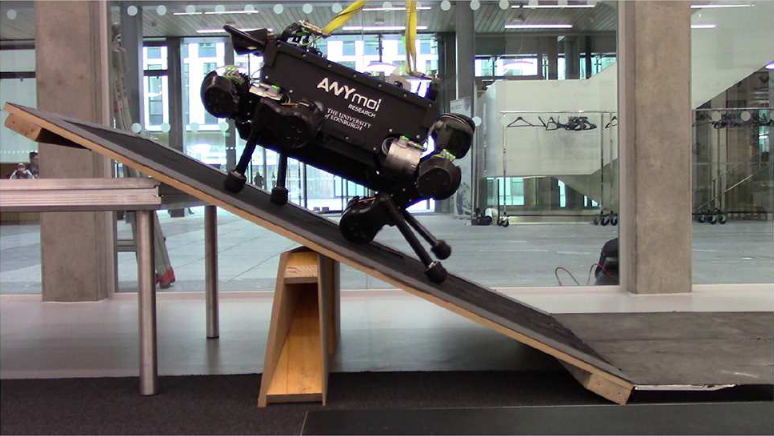
\includegraphics[height=0.27\columnwidth]{anymal.pdf}
		\label{subfig:anymal}}
	\subfloat[]{
		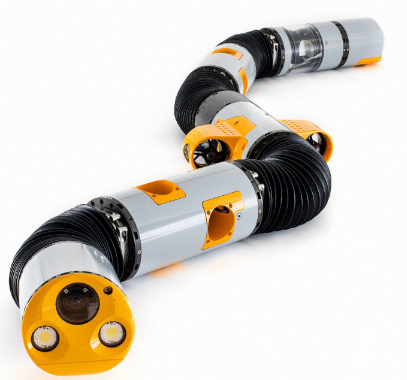
\includegraphics[height=0.27\columnwidth]{snake}
		\label{subfig:snake}}
	\hfil
	\subfloat[]{
		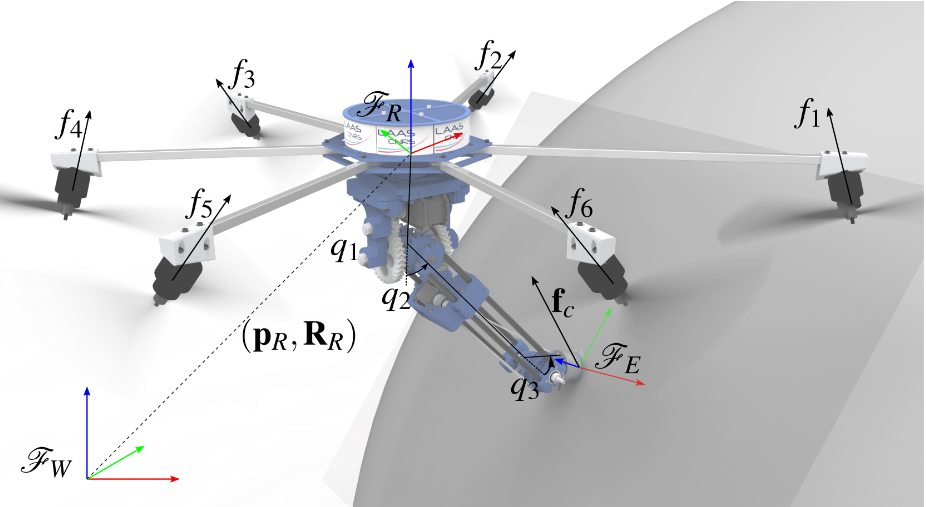
\includegraphics[width=0.478\columnwidth]{aerialManip.pdf}
		\label{subfig:aerialManip}}
	\subfloat[]{
		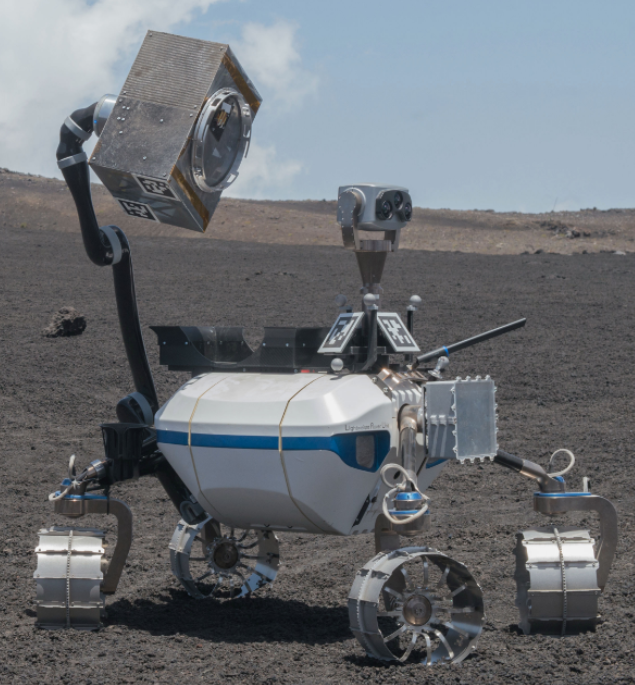
\includegraphics[height=0.27\columnwidth]{rover}
		\label{subfig:rover}}
	\subfloat[]{
		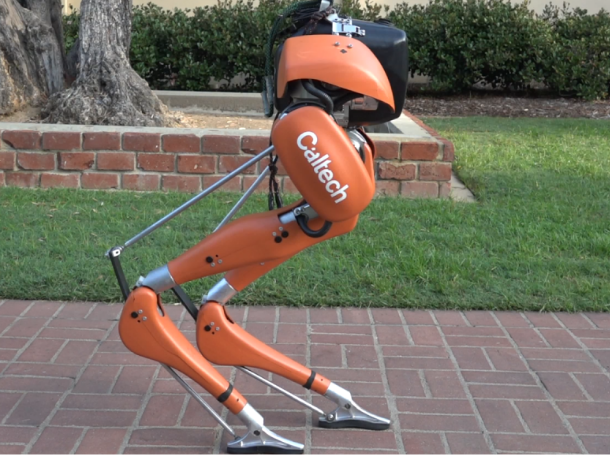
\includegraphics[height=0.27\columnwidth]{cassie.pdf}
		\label{subfig:cassie}}
\caption{Different robotics platforms controlled with multi-objective QP.~\subref{subfig:hrp4_double} Humanoid~\cite{djeha2020ral}.~\subref{subfig:anymal} quadruped~\cite{xin2020frontiers}.~\subref{subfig:snake} Snake-like robot~\cite{basso2020ifac}.~\subref{subfig:aerialManip} Aerial manipulator~\cite{nava2020ral}.~\subref{subfig:rover} Planetary rover~\cite{bussmann2018icra}.~\subref{subfig:cassie} Bipedal~\cite{reher2020acc}.}
\label{fig:QP controlled robots}
\end{figure}

\subsection{Multi-Contact, Balance and Locomotion}
Beyond free-space motion, robots are often required to establish contact with their environment for keeping balance, locomotion, or applying a desired force. 
Establishing contact with a predefined desired force can be achieved either by direct force control or admittance control~\cite{pham2020ral}.~\cite{nava2020ral} formulated a QP controller for an aerial manipulator interacting physically with the environment to perform highly dynamic motion. To mitigate the planning process burdens on dealing with potential collisions, \cite{pang2021arxiv} proposed contact-aware QP controller. The latter tracks joint reference trajectories while online servoing  frictional forces due to unexpected contacts to predefined operator-defined values. 

Multi-objective QP  showed great efficiency on graphical animation of bipedal characters performing human-like whole-body motion while accounting for frictional contact forces, non-coplanar contacts, bilateral grasping, and balance~\cite{abe2007siggraph,delasa2010trGraph,collette2007humanoids}. 
Motivated by these works, QP has been formulated to control the balance of humanoid robots. Due to their underactuation,  humanoid robots need to rely on the contact forces to act on the floating-base (and subsequently, the CoM). In order to achieve balance, the contact forces and joint torques have to compensate for all dynamics that apply to the robot in terms of inertia, gravity, and external disturbances. QP can then be formulated to exploit the robot redundancy to fulfill the frictional constraint on the forces to avoid slipping or losing contacts while tracking the desired tasks references. This has been achieved using the soft-hierarchical~\cite{righetti2012humanoids,righetti2013ijrr} and strict-hierarchical~\cite{sherikov2015humanoids} schemes. 
%QP has been formulated to control the balance of humanoid robots in multi-contact scenarios while accounting for other constraints particularly hardware limitations and collision avoidance. For instance, maintaining balance through optimal contact-forces distribution has been formulated using soft-hierarchical~\cite{righetti2012humanoids,righetti2013ijrr} as well as strict-hierarchical WBQP~\cite{sherikov2015humanoids}. %can be formulated b to control the balance of humanoid robots in multi-contact scenario by following either a soft or strict hierarchy~\cite{righetti2012humanoids,righetti2013ijrr,sherikov2015humanoids}. 

The contacts can be planned along with the corresponding postures. Then, the QP controller computes the control inputs to satisfy the frictional contact forces, collision avoidance, and torque limits while converging at best to the desired task-states. This method allows performing complex multi-contact scenarios. It has been applied for ladder climbing in~\cite{vaillant2016springer}, getting through narrow passages, and ingressing into a car cabin~\cite{bouyarmane2012humanoids_b}.%, QP is proposed for multi-contact ladder climbing using HRP-2 humanoid robot. QP tracks the desired tasks' references forwarded by FSM based on a posture-in-contact generator.
~\cite{samadi2021ral} studied the question of how to ensure real-time balance while switching between fixed and sliding non-coplanar multi-contacts. The authors proposed a centroidal QP based on the Chebyshev center that computes the optimal contact forces distribution and the CoM location. These optimal targets are then tracked by whole-body QP using admittance task~\cite{bouyarmane2019tro}.~\cite{herzog2016autonomousRobot} proposed to control the balance of bipedal robot Sarcos by formulating a momentum-based real-time hierarchical QP. The approach enabled balancing the robot on double and single support while being robust to external disturbances. Ensuring balance for a wheeled inverted-pendulum robot, like Ninebot Segway, is even more challenging. In~\cite{gurriet2018iccps}, a balance strategy consisted of constraining the pendulum angle using CBF-QP formulation to remain in a small bounded set around zero to keep it upright.


%\subsection{Visual Servoing}

%\subsection{Model Predictive Control}


%The emergence of humanoid robots raises new challenges in term of locomotion and multi-contact establishing to maintain balance.  Motivated by these works, QP has been exploited to control the balance of humanoid robots in multi-contact scenario by finding the optimal contact-force distributions following either soft or strict hierarchy~\cite{righetti2012humanoids,righetti2013ijrr,sherikov2015humanoids}. 
A walking trajectory generator is necessary for bipedal locomotion to provide feasible CoM trajectories based on the footstep plan. The latter are then tracked by QP while tracking the feet-swing trajectory and ensuring frictional contact forces~\cite{englsberger2018icra,koolen2016ijhr,kuindersma2016autonomousRobot}.   
For stair climbing,~\cite{caron2019icra,kheddar2019ram} formulated a QP layer on top of whole-body QP to distribute the net wrenches (that corrects the CoM position and velocity) at the contact points while satisfying contact stability\footnote{to not confuse with the stability notion in Lyapunov sense, see~\cite{caron2017tro}.}. 
\subsection{Impacts}
Contacts can also be performed with the environment with a non-zero contact velocity resulting in impacts. Impacts frequently occur for humans like grabbing an object, drumming, hammering, jumping, etc. However, impacts are particularly challenging for QP controllers as the resulting joint-velocity jump may lead to an aggressive reactive response or even to an empty feasible domain. QP-based approaches focused either on minimizing the joint velocity jump assuming one-step-ahead impact prediction~\cite{wang2019rss} or by projecting the control objectives into an impact invariant subspace~\cite{yang2021iros}. 

Impacts with deformable objects have also been studied. Due to the post-impact object soft deformation, the pre-impact robot motion is less restricted~\cite{dehio2021icra}. In~\cite{dehio2022ral}, a QP controller has been formulated to control soft-pads dual-arm robots for object grabbing. QP tracks the end-effector velocity targets computed by a Model Predictive Controller (MPC) on top of QP to predict deformation trajectory while accounting for the robot joint bounds and hardware limitations. 

Handling impacts generated when walking can be performed with the hybrid theory since bipedal robots (seen as hybrid systems) go through continuous and discrete dynamics. Cyclic bipedal walking has been formulated using CLF-QP to ensure rapid-exponential stabilization of MABEL bipedal robot periodic gait~\cite{ames2012cdc,ames2014tac}.

\subsection{Safety and Human-Robot Interaction}
Ensuring safety is critical for most robotic applications. The safety concerns the robot (hardware and structure), its surrounding environment, human operators, and other robots. A safety-critical controller is then required to keep the robot state away from the unsafe configurations or, equivalently, to render the set of safe configurations invariant.%So far, CBF-QP  framework shows up as a suitable tool to synthesize these type of controllers, while tracking desired trajectories.   

Safe adaptive-cruse controller has been proposed in~\cite{xu2017ccta,ames2014cdc,ames2017tac} and formulated using CBF-CLF-QP. QP regulates the car velocity to move with the desired velocity while not crashing with the car in front and controlling the steering to keep the lane. This policy has been applied  in~\cite{wang2017tro} to avoid collisions between wheeled robots in a swarm configuration. Centralized and decentralized QP formulations have been proposed showing interesting behaviors of the agents when they are: (i) controlled with a single controller (similarly to the multi-robot QP in~\cite{bouyarmane2019tro}); and (ii) controlled individually. This formulation can also be a good tool for modeling individuals' behavior  responding to a given stimulus. The same formalism has been applied in~\cite{wang2017icra} to rectify the preplanned quadrotors' trajectories if they lead to collision during the flight. 

For legged robots, the safety aspects can encompass safe foot placement on the predefined footholds~\cite{nguyen2016cdc,nguyen2016acc2,grandia2021icra}, avoiding surrounding obstacles and self-collisions~\cite{molnar2022ral,vaillant2016trvcg,quiroz-omana2019ral}, keeping the CoM inside equilibrium region and joint limits satisfaction~\cite{djeha2020ral}. 

In~\cite{rauscher2016iros,murtaza2022ral}, safe robot motion in a confined Cartesian space is performed by exploiting redundancy and CBF to avoid collision with virtual boundaries. The latter are learned by demonstration in~\cite{saveriano2019iros} allowing the operator to specify and customize the safety boundaries easily for the robot directly at the workspace.

Safe human-robot interaction has also been studied since humans and robots increasingly share the same workspace. In~\cite{landi2019ecc,ferraguti2020ras}, CBF-based collision avoidance constraint is introduced to QP to prevent the robot from impacting the human operator. The relative distance between the two agents is computed based on the primitive geometric models of the human and robot multi-bodies. Alternatively, 
the robot's kinetic energy is a reasonable metric to monitor how harmful the robot could be. In~\cite{meguenani2016iser,joseph2018iser}, a constraint is formulated to upper bound the kinetic energy. This constraint limits the kinetic energy dissipation in the case of an unexpected impact. If the maximum allowed kinetic energy is set to zero, then the joint velocity must also drop to zero. Since this change cannot be achieved instantaneously from any initial velocity due to the joint acceleration and jerk limits,~\cite{joseph2020iros} proposed a safe-braking constraint on the joint velocity that accounts for the latter limitations and  the relative distance between the human and robot.   

Interaction between human and robot has been shown to be adequately cast to multi-robot QP paradigm where the human is considered as a multi-body robot~\cite{bolotnikova2020roman,bolotnikova2021sii}. For instance, frail persons' conditions can be easily simulated with a human model with low joint-torque abilities. This formalism enables to elaborate systematic approaches for humanoid-to-human assistance
and whose performances can be quantitatively and qualitatively measured~\cite{bolotnikova2021ral}. Human-robot handovers also constitute an essential and frequent form of interaction. Based on multi-robot QP, the handover has been shown to be nicely formulated by considering the object to be exchanged as a rigid-body robot whose pose, velocity, and acceleration are estimated via an observation task unified with the tracking task~\cite{djeha2022arxiv}. This is the topic of \cref{chap:handover qp}.  

\subsection{Visual Servoing and Observation}
Mounting cameras on articulated robots appealed for an elaborated technique to merge visual servoing and redundancy resolution control. The first use of QP for this purpose was performed in~\cite{ellekilde2007ijars} where the camera was mounted on a redundant robot arm end-effector. QP enabled a fast visual servoing while avoiding joint limits and singular configurations. Thanks to the natural handling of inequality, visual servoing QP has been formulated to account for FoV constraint and occlusion avoidance~\cite{agravante2017ral}. The same approach has been applied in~\cite{chen2021sensors} for quadrotor control to visually track a vehicle on the ground and keep it within the FoV bounds.  

Another significant usage of visual servoing is the observation of a given state to be regulated by QP via error feedback.  
This idea has been applied in~\cite{paolillo2014humanoids,paolillo2018fieldRobotics} where a strategy has been drawn to drive a car reactively by a humanoid robot. Visual servoing has been performed to detect the road features and estimate the car velocity leveraging other onboard sensors. In~\cite{tanguy2019icra}, simultaneous localization mapping has been used to estimate the location of humanoid CoM to accurately replan the CoM trajectories via MPC to maintain balance even under external disturbances.  
To mitigate the question of estimating the configuration of a passive articulated object (door, draw, valve wheel, etc),~\cite{paolillo2017sii} proposed the concept of virtual visual servoing. It consists of defining a virtual object that converges to the real one allowing to estimate implicitly real object configuration. The virtual visual servoing has been defined as a task in QP in~\cite{paolillo2018fieldRobotics} which accounts for the object constraints. 

Rather than estimating a state to achieve the control feedback, the observation can also be performed to estimate a target for a given task. This idea has been proposed in~\cite{djeha2022arxiv} to estimate the full-state of an object (in terms of pose, velocity, and acceleration) when only the pose is accessible for measurements. These estimated states are then the feedforward target terms of a trajectory tracking task. This concept has been applied to human-robot handover to ensure the robot and object meeting without prior knowledge of the object exchanging location. Conversely to~\cite{paolillo2018ral}, the observation is fully-fledged as a task in multi-robot QP, and it is not dependent strictly on visual servoing. 

\cite{agrawal2022csl} considered the safety of systems subject to disturbances in the dynamics as well on the state measurements. More importantly, the authors addressed the case where the state is only partially measured, thereby requiring an observer to construct the full-state. A robust CBF-QP has been proposed to enforce the system's safety while accounting for the state estimation error. These controllers result typically in confining the system trajectories inside a more restrictive set similarly to~\cite{kolathaya2019csl,alan2022csl}. However, this can be very conservative, especially that the CBF design requires the knowledge of some parameters that cannot be known precisely in practice. 

\section{Conclusion}
%After that, we presented the different multi-objective control schemes that can be performed using QP by stating the pros and cons of each control scheme.

In particular, we highlighted the current efforts in the research community to address the still open question in the QP control paradigm. More concretely, kinematic constraints formulation, stability and robustness of the closed-loop QP control, constraints compatibility, and how to unify control and observation. Each of these points is  addressed in a dedicated chapter. 

In the next chapter, we  present our first contribution in this thesis about kinematic constraints formulation to be enforced by the decision variables. We consider the case when the kinematic constraints are online introduced to QP as explained in~\cref{subsubsec-chap0:online constraints introduction}. Rather than using BF theory, our formulation is analytical and based on ODI with adaptive gains allowing us to prove formally the forward invariance and asymptotic stability of the kinematic constraint set. 
%Driving a car is a typical process that requires visual servoing combined with other command actions like the steering and the acceleration. Visual servoing mainly detects the road features and estimates the car velocity using the on-board sensors
%\cite{paolillo2018fieldRobotics} demonstrated the ability of a humanoid robot to reactively drive a care in different control modes: total, partial, or shared autonomy. The visual servoing detects the road features and estimates the car velocity using the on-board sensors~\cite{paolillo2014humanoids}. Then, a multi-objective QP controls the ankle angles on the gas pedal to track the desired car velocity, and the hand to move the steering wheel to keep the car within the detected road edges. %  the has been formulated to control 

%Visual servoing is inherently related to observation. In particular, manipulating passive articulated objects (door, draw, valve wheel, etc) by a robot requires the estimation of the object configuration. Leveraging multi-robot QP where a printer is considered as a floating-base robot and one passive DoF,~\cite{paolillo2017sii} estimated the position of the printer drawer using virtual visual servoing. This concept consists on defining a virtual object that converges to the real one allowing to estimate implicitly real object configuration. In~\cite{paolillo2018ral}, the virtual visual servoing has been defined as a task and integrated in QP.  

%Following the same architecture,~\cite{samadi2021ral} implemented a centroidal QP layer for contact force distribution and suitable location for CoM to ensure balance while switching between fixed and sliding contacts. % In~\cite{caron2019icra}, QP has been formulated for contact wrench distribution to satisfy contact stability.  %Generally, the contact locations and the associated wrenches are synthesized by a planner. The multi-objective whole-body QP has been used to optimally solve the redundancy while reaching the contact location and applying the desired wrenches  

%\subsection{Kinematic-Controlled Robots}
%In~\cite{hu2014icra}, a position-dependent velocity constraint is proposed to avoid QP failure when the humanoid robot knees are fully stretched while walking. The same formulation is given in~\cite{flacco2015tro} for redundant robotic manipulators. This constraint is also known as \textit{viability constraint} in~\cite{delprete2018ral}, where a discrete-time implementation in terms of joints acceleration is provided.
%All these approaches have the following shortcomings (explicitly acknowledged by their authors):
%\begin{itemize}
%	\item A precise knowledge of the robot state is necessary and hence assumed;
%	\item Undesirable discontinuous motions (chattering) near the constraints bounds in closed-loop;
%	\item Mostly applied for joints bounds and few in collision avoidance;
%	\item They do not handle time-varying bounds.
%\end{itemize}

%\section{Cobots}
